%%%%%%%%%%%%%%%%%%%%%%%%%%%%%%%%%
% thesis.tex: This is the Primary TeX control file for thesis.
%%%%%%%%%%%%%%%%%%%%%%%%%%%%%%%%%

%%%%%%%%%%%%%%%%%%%%%%%%%%%%%%%%%%%%%
%%% 
%%% CHANGE TO MNTHESIS CLASS'S DEFINITION OF XFLOATS.
%%% 
%%% This change allowed me to use the deluxetable environment, which is what
%%% my Tables were (already) made in for the AJ articles.  One of the tables
%%% is both rotated and contains footnotes, which deluxetable can do but
%%% which the other table environment included by default in the MN thesis
%%% template could not handle.
%%%
%%% I learned this fix from:
%%% 		http://tex.stackexchange.com/questions/191808/problems-with-tikz-when-i-change-document-class
%%%
%%% save a copy of the kernel's \@xfloat
\makeatletter\let\latex@xfloat\@xfloat\makeatother
%%%
%%% load the mnthesis class
\documentclass[11pt,oneside]{mnthesis}
%%%
%%% fix floats to use single spacing
\usepackage{etoolbox}
\makeatletter
\let\@xfloat\latex@xfloat
\apptocmd{\@xfloat}{\linespread{1}\normalsize}{}{}
\makeatother
%%%
%%% (END OF CHANGE TO MNTHESIS CLASS'S DEFINITION OF XFLOATS.)
%%%%%%%%%%%%%%%%%%%%%%%%%%%%%%%%%%%%%%


\usepackage{epsfig,epic,eepic,units}
\usepackage{hyperref}
\usepackage{url}
\usepackage{longtable}
\usepackage{mathrsfs}
\usepackage{multirow}
\usepackage{bigstrut}
\usepackage{epigraph}
\usepackage{amssymb}
\usepackage{amsmath}
\usepackage{graphicx}
\usepackage{textcomp}
\usepackage{threeparttable}

% Per Jake Simones' github notes, this packages aastex_hack from Pete Mendygral
% eases the use of common AASTeX commands
\usepackage{aastex_hack}

\usepackage{natbib, deluxetable}

% add this package for subfigures
\usepackage[caption=false]{subfig}   

\linespread{1.3}		% not sure what this does, but it's in the MN template

\begin{document}

% Bibliography style file: I changed from the template's default to the apj style file ``apj.bst'' because hunrst.bst did not
% format the cites in the text the way they should be.  
\bibliographystyle{apj}

% Title and the other sections that appear before the body of the document (List of Figures, List of Tables)
%%%%%%%%%%%%%%%%%%%%%%%%%%%%%%%%%%%%%%%%%%%%%%%%%%%%%%%%%%%%%%%%%%%%
% title.tex - Set up the beginning of thesis.
%%%%%%%%%%%%%%%%%%%%%%%%%%%%%%%%%%%%%%%%%%%%%%%%%%%%%%%%%%%%%%%%%%%%
% For a  PhD give the command \phd. Default is masters
%\degree (normally Doctor of Philosophy or Master of Science)
%\initials (normally Ph.D. or M.S.)
%\ms % use if for a Master of Science thesis
\phd % use if for a Ph.D. dissertation
% \draft

\title{\bf Morphology is a Link to the Past: examining formative and secular galactic evolution through morphology}
\author{Melanie A. Galloway}
\campus{University of Minnesota} 
\program{Physics} 
\degree{Doctor of Philosophy}
\director{Advisor:\\ Lucy Fortson} 

% Optionally specify the month and year.
\submissionmonth{August} % defaults to current month.
\submissionyear{2017} % defaults to current year.

%Comment out below on final copy
\abstract{%%%%%%%%%%%%%%%%%%%%%%%%%%%%%%%%%%%%%%%%%%%%%%%%%%%%%%%%%%%%%
% abstract.tex: Abstract
%%%%%%%%%%%%%%%%%%%%%%%%%%%%%%%%%%%%%%%%%%%%%%%%%%%%%%%%%%%%%

%Galaxies are cool and have pretty colors sometimes. Can I has degree now? Thx :)

%\bigskip 

Galaxy morphology is one of the primary keys to understanding a galaxy's evolutionary history. External mechanisms (environment/clustering, mergers) have a strong impact on formative evolution of the major galactic components (disk, bulge, Hubble type), while internal instabilities created by bars, spiral arms, or other substructures drive secular evolution via the rearrangement of material within the disk. This thesis will explore several ways in which morphology may impact the dynamics and evolution of a galaxy using visual classifications from several Galaxy Zoo projects. Section 1 will focus on the present morphology of galaxies in the local Universe ($z<0.2$) using data from Galaxy Zoo 2 and Galaxy Zoo UKIDSS. Section 2 will examine populations of morphologies at various lookback times, from $z=0$ out to $z=1$ using data from Galaxy Zoo Hubble.


%%GZ2 bar/agn study
We first explore the impact of bars in disc galaxies on channeling gas from the outer regions of the disk to the inner few kpc necessary to fuel an active galactice nucleus (AGN). Using a sample of 19,756 disk galaxies at $0.01 < z < 0.05$ imaged by the Sloan Digital Sky Survey and morphologically classified by Galaxy Zoo 2, the difference in AGN fraction in barred and unbarred disks was measured. A weak, but statistically significant, effect was found in that the population of AGN hosts exhibited a 16.0\% increase in bar fraction as compared to their unbarred counterparts at fixed mass and color. These results are consistent with a cosmological model in which bar-driving fueling contributes to the fueling of growing black holes, but other dynamical mechanisms must also play a significant role. 

%%study/results of GZ UKIDSS
We study the wavelength dependence on morphology by comparing the optical morphological classifications from GZ2 to classifications done on infrared images in GZ:UKIDSS. We find some cool result. [to be continued]

% study/results of GZH science
We examine more directly the morphological changes in galaxy populations as a function of their age using classifications from Galaxy Zoo: Hubble. A sample of XX,XXX disc galaxies from the COSMOS field at $0<z<1$ were identified as active or passive using a NUV-r / r -J diagnostic with rest-frame colors from the UltraVISTA catalog. We find that the fraction of disks that are passive increases/decreases from X.X\% at $z=1$ to X.X\% at $z=0$. We intepret this result as [something having to do with the transformation of disk to elliptical, depending on result]. Addionally, we emphasize the challenges of visual classification that are particular to galaxies at high redshift. We present a correction technique to address these biases using simulated images of nearby SDSS galaxies which were artificially redshifted using the FERENGI code and classified in GZH.  








}
\words{331}    % number of words in the abstract
\copyrightpage % Do you want copyright protection?
\acknowledgements{% acknowledge.tex: Acknowledgements




}
\dedication{% dedication.text

Firstly dedicated to Zuko, for being the sweetest little bird. 
}

% Use a special preface
%\extra{\input{preface}}

% The \beforepreface command actually causes insertion of the title, 
% abstract, signature, and copyright pages into the new document.
\beforepreface 

% Define the text to go before the table of contents
\figurespage
\tablespage

% The \afterpreface command actually causes insertion of the
% contents, list of figures, etc. into the new document.
\afterpreface            
%%%%%%%%%%%%%%%%%%%%%%%%%%%%%%%%%%%%%%%%%%%%%%%%%%%%%%%%%%%%%%%%%%%%%%%%%%%%%%%%


% Intro Chapter
%%%%%%%%%%%%%%%%%%%%%%%%%%%%%%%%
% intro.tex: Introduction to the thesis
%%%%%%%%%%%%%%%%%%%%%%%%%%%%%%%%
\chapter{Introduction}
\label{chap:intro}

The Intro
reminder to include: discussion on wavelength-dependence of morphological classifications. Discuss the transition of star formation coming through in optical, disappearing in near-IR, then reappearing in mid-IR (Galaxy Morphology Buta 2013 and briefly at end of Buta 2010). 

Super inspiring first paragraph. Segue: now we'll take a moment to breifly introduce/describe/define important morphologial types. 

\section{Morphological Categorization of Galaxies}

The oldest and most well-known system which categorizes galaxies based on their structure was developed by Edwin Hubble, commonly known as the ``Hubble Tuning-Fork'' \citep{Hubble1926}. Using a small sample of photometric images of nearby galaxies, Hubble identified two fundamental morphological classes: spirals, which exhibited well-defined disk structure and clear spiral arms, and ellipticals, whose light distributions were smoothed over a roughly spherical shape. Only 3\% of the sample had structures which deviated from these two categories, showing no evidence of rotational symmetry about a dominating nucleus; these were grouped together and labeled ``Irregular''. Although Hubble's system was originally based on a mere 400 galaxies, the classifications are still valid for describing the morphologies of the millions of galaxies identifiable today (albeit with some modications, ie. DeVaucouleur's revised system \citep{DeVaucouleurs1963}).

An example of Hubble's Tuning Fork is shown in Figure \ref{fig:tuningfork}. The classifications defined on the Tuning Fork are as follows:

\begin{figure}
\centering
\includegraphics[width=\textwidth]{figures/TuningForkKaren.jpg}
\label{fig:tuningfork}
\caption{The Hubble Tuning fork with gri-composite SDSS images as examples of the various types. Credit: Karen Masters and The Sloan Digital Sky Survey (SDSS) Collaboration.}
\end{figure}

\subsection{Ellipticals}

The left side of the tuning fork contains elliptical galaxies, labeled ``E''. These were originally identified as circular through flattened ellipses whose luminosity faded smoothly from the center to ``indefinite edges.'' The only other structural feature evident to subdivide this class were their ellipticities, defined in the traditional way $e=(a-b)/a$. A number is added to the label that represents the ellipticity, with the decimal omitted, whereby E0 would represent a purely spherical elliptical ($e=0$), and E7 being the most elongated ($e=0.7$). Hubble assumed that any galaxy with an ellipticity higher than 0.7 was no longer an elliptical, but more likely a highly-inclined spiral. It should be noted that these labels only classify the \emph{projected} appearance; since ellipticals are tri-axial structures, this classification system is very dependent on the orientation angle of any ellipticals which are not perfectly spherical.  

\subsection{Spirals}

The right side of the fork contains the various types of spiral galaxies. These all share the feature of having a flattened disk-shape, and tend to have a spherical bulge of stars in the center with spiral arms extending outward. Spirals whos arms originate from the central bulge follow the top of the fork, labeled ``S'', while those whose arms originate at the ends of a central galactic bar follow the bottom, labeled ``SB''. Both types are further classified based on the relative size of the central bulge and tightness of the arms. Those with large bulges and tighter arms are designated with an ``a'' attached to the spiral symbols, or ``b''-``d'' for decreasing bulge sizes and looser appearance of arms. 

\subsection{Lenticulars/S0s}

Lenticular galaxies are placed at the center of the tuning fork, originally thought to be a transition stage to link the elliptical and spiral types. They exhibit the same overall disk-shape as the spirals, but have a smooth appearance rather than defined arms (which can make them difficult to distinguish from true ellipticals). They may or may not contain a galactic bar, giving them Hubble-type classifications of S0 (unbarred) or S0B (barred). 


Hubble originally referred to the galaxies toward the left and right on the fork as ``early'' or ``late''-type, respectively, simply for convenience in describing their relative positions on the sequence. While it is noted in his 1926 paper that any temporal connotation should be disregarded, the terms remain misleading in that it is now well-known that the early types tend to have older stellar populations, and late-types tend to be very young in their evolution. Nevertheless, ``early-type'' and ``late-type'' are still today used interchangeably when referring to ellipticals/S0s and disks. 

\section{Morphology as a tracer of galaxy evolution}

The previous section described the most common morphological types of galaxies observed in the Universe. At this point it may be relevant to question, why are there different types at all? Do the different shapes exhibit different evolutionary pathways, or is the snapshot we see of the distributions simply showing different stages of a track that all galaxies eventually follow? The answers to these questions aren't fully known; however, examining the relationships between the different morphological types and their dynamics can provide strong insights to the full picture. This section will provide some examples of well-known links between morphology and galaxies' evolutionary histories.

\subsection{Color-Morphology Bimodality}

The color of a galaxy is a strong indicator of its recent star formation history. In general, photometrically blue galaxies are in the process of forming new stars, emitting high energy blue light that is detected abundantly in short-wavelength filters. In contrast, galaxies which have ceased forming stars sometime in the past contribute most of their flux to long-wavelength filters, resulting in redder colors. Perhaps surprisingly, there is also a strong correlation between the color of a galaxy and its morphology. The majority of galaxies ($\sim80\%$) have been shown out to $z\sim1$ to follow this relationship: blue galaxies tend to be late-type spirals, and red galaxies tend to be early-type/elliptical \citep{Tully1982,Strateva2001,Baldry2004,Conselice2006,Martin2007,Mignoli2009}. An example is shown in Figure~\ref{fig:cmd}. The vertical axis tracks the $u-r$ color, such that higher values are ``redder'' and smaller values are ``bluer''. Bluer galaxies tend to have more featured morphologies; spiral arms appear more flocculant and clumps of star formation are apparent, generating irregular shapes in the extreme cases. Redder galaxies begin to have a much more smoothed-out and symmettric appearance, encompassing both ellipticals and bulge-dominated lenticulars. Color has long been considered such a strong indicator of morphology that it has been often used as a proxy for morphology when large-scale visible inspection has not been practical \citep{Cooray2005,Lee2007,Salimbeni2008,Simon2009}. This link is strong evidence that the processes which drive both morphology and the cessation of star formation are related in some way \citep{Masters2010,Buta2013}. This topic is explored in greater detail in Chapter~\ref{chap:gzh_red_disks}. 

\begin{figure}
\centering
\includegraphics[width=\textwidth,trim={3cm 3cm 6cm 3cm},clip]{figures/sdss_plot.pdf}
\label{fig:cmd}
\caption{Color vs. Absolute Magntitude Diagram, illustrated using SDSS galaxies. In each color-magnitude bin, a random galaxy was selected meeting the criteria defined by that bin.}
\end{figure}

\subsection{Morphology and Environment}

A galaxy's environment can also be a predictor of its morphology. The morphology-density relationship, first quantified by \citet{Dressler1980}, observes an abundance of elliptial/early-type morphologies in denser environments \citep{deSouza1982,Postman1984}. Since the merger rate correlates with environment density, it could be suggested that early-types are often the by-products of mergers, as opposed to a stage of isolated secular evolution. 

There is also evidence of an environmental impact on morphology even in the absence of direct merging. For example, ram pressure \citep{Gunn1972} exerted by the local intracluster medium can severly distort the gas distribution in a galaxy, resulting in asymmetries in the disk (ex. NGC 4402; see also Chapter~\ref{chap:gzh_red_disks}).  

\subsection{Bars}
\citet{Buta2013} describes barred galaxies as ``the ultimate in galaxy morphology.'' His reasoning is simple: just by observing an image of a bar, it is easy to identify it as a major perturbation in an otherwise stable system. There is a great deal of truth in this; such a disruption will no doubt have profound effects on the fate of its host galaxy. In this way, bars are arguably one of the most important structural features that can shape a galaxy's evolution. 

A key feature of bars is their ability to drive gas from the outer regions of the galaxy to the center \citep{Athanassoula1992,Friedli1993,Ann2005,Kormendy2004,Athanassoula2005,Sellwood1993,Shlosman1989}


\section{Methods for morphological classification}

Historically, most methods of morphological classification been done by visual inspection of small samples of images (e.g. \citet{Hubble1926,Sandage1961,DeVaucouleurs1963,Block1994,Eskridge2002,Buta2010}), by either a single person or handful of experts. This method is becoming obsolete as we enter a new era of large data, with recent surveys such as SDSS and HST-Legacy, and upcoming JWST and LSST, producing high-quality images of hudreds of thousands of galaxies. To date, the largest morphological catalogs created by visual inspection from a small group of experts includes the Nair and Abraham catalog \citep{Nair2010} with $\sim$ 14,000 galaxies, RC3 Catalog \citep{RC31991} with $\sim$ 23,000 galaxies, and MOSES \citep{Schawinski2007} with 50,000 galaxies. Even these catalogs, while successful, do not compare in size to the newly incoming data, and so more powerful and robust efforts are required to obtain morphological information on these scales.

One alternative to direct visual classification of morphologies is the use of proxies such as color, mass, surface brightness profile, or some combination of several. Color is commonly used as a proxy because of its mostly-tight relationship global morphology, in that spirals tend to be red and ellipticals tend to be blue. This type of morphological classification will always suffer from a high degree of inaccuracy, as there is no perfect physical measurement that is 100\% correlated with shape. The morphology of a galaxy traces the dynamical history, where proxies such as color trace stellar growth; these two properties thus reveal different evolutionary histories on possibly very different timescales \citet{Fortson2011}. Last, while there are several proxies which correlate somewhat with the probability of a galaxy being spiral or elliptical, very few could be used to identify finer substructures or more detailed morphological features within the overall shape. 

An ideal method for handling the large amounts of data would be an automated classification scheme. Several such algorithms have been developed, with some success \citep{Odewahn2002,Peng2002,Conselice2003} by using the stellar light distribution of the galaxy to assign it a morphological class. These approaches tend to be limited to identifying the global morphologies (ie, spiral or elliptical), and lack the precision to accurately identify finer, detailed features (such as bars or the number of spiral arms) (Beck et al. 2017). Further, they tend to incorporate proxies such as color as their input, which are often not accurate as previously noted. Much more promising techniques are currently being tested which incorporate the use of machine-learning algorithms and neural networks \citep{Dieleman2015, Huertas-Company2015},(Beck et al.2017), but these require massive and accurate training-sets to perform properly. 

A best-of-both-worlds approach uses the power of crowdsourcing, which uses the input of thousands of individuals to visually classify galaxies in a fraction of the time achievable by a handful of experts; such a method was developed by Galaxy Zoo, the data from which is used throughout this thesis. The Galaxy Zoo project uses a simple online interface whereby images of galaxies are visually inspected by volunteers, which allows the identification of intricate morphological features to a higher degree of accuracy than computer algorithms today can achieve. Addionally, with a required 40+ independant classifications per galaxy, the resulting classifications carry a greater statistical significance than those generated from one or a few experts. The next chapter will describe how Galaxy Zoo collects data from volunteer citizen scientists, how the data is reduced and debiased, and finally how the data is used to assign morphological classifications to large samples of galaxies.  


% end of chapter








% The main Chapters
%%%%%%%%%%%%%%%%%%%%%%%%%%%%%%%%
% methodology.tex: Citizen Science chapter
%%%%%%%%%%%%%%%%%%%%%%%%%%%%%%%%
\chapter{Methodology}
\label{chap:methodology}

\section{A Brief History of Galaxy Zoo}

The increasing accessibility of the Internet in the last decade has allowed scientists to ``outsource'' tasks online using citizen science, with huge success. The project Seti@Home \footnote{http://setiathome.berkeley.edu/} \citep{Anderson2002}, launched in May 1999, was one of the first projects that revealed the massive number of people willing and excited to help contribute to science. Since launch, over 5 million participants donated idle time on their computers to assist SETI in analyzing radio telescope data to help in the search for extraterrestrial life. Citizen scientists were also extemely interested in taking in an even more active role in research, as seen in a later project Stardust@Home \footnote{http://stardustathome.ssl.berkeley.edu/}, in which volunteers searched for dust grains in data via a web interface. This project engaged over 20,000 volunteers, and those who discovered dust grains were invited to become co-authors on the announcement papers. Early citizen science projects such as these inspired the launch of Galaxy Zoo.

The real need for a faster method of obtaining galaxy morphologies for large samples was realized in 2007 by graduate student Kevin Schawinksi, who was studying populations of elliptical galaxies as work for his PhD thesis at Oxford University. At the time, the accepted and fastest method for identifying early-type galaxies (in large quantities) was to select based on SDSS-measured spectra \citep{Bernardi2003}. He knew, however, that this sort of method would exclude potential star-forming ellipticals (as well as potentially include passive spirals), due to the non-perfect correlation between morphology and color, as mentioned in the previous Chapter. So, realizing that a visual inspection of the direct appearance of the galaxies was necessary to create a complete sample of ellipticals independent of color, Schawinksi devoted an entire week to classifying 50,000 galaxies by eye (MOSES, \citet{Schawinski2007}). 

The grueling task of classifying only a small fraction of the entire SDSS main sample ($\sim$ 900,000 galaxies) made it apparent that a better method for visual classification was becoming neccessary. Inspired by the 20,000 volunteers who participated in the Stardust@Home project, Schawinksi and Oxford colleague Chris Lintott realized that it would only take a few years to classify all of SDSS Main, assuming a similar participation response as StarDust. This led to the launch of Galaxy Zoo in July, 2007. This first phase (known now as Galaxy Zoo 1, or GZ1), included the brightest (Petrosian magnitude $r < 17.77$ AB mag) 893,212 images from SDSS Data Release 6 \citep{Strauss2002,AdelmanMcCarthy2008}. In this project users were asked to indentify simple features of a given galaxy, including whether it was elliptical or spiral, clockwise or anticlockwise, a merger, or star/other (the original interface with options is shown in Figure~\ref{GZ1_Interface}. 

\begin{figure}
\centering
\includegraphics[width=.8\textwidth]{figures/GZ1Interface.png}
\caption{GZ1Interface}
\label{GZ1_Interface}
\end{figure}

In just the first day of the site being live, 20,000 classifications were coming in each hour - a rate much faster than the developers had ever expected. In less than a year, the entire SDSS main sample was classified by an average of 38 volunteers per galaxy. Following GZ1 data release paper published in April, 2008 \citep{Lintott2008}, over a dozen scienific publications were released which made use of the morphological classifications \footnote{https://www.zooniverse.org/about/publications}. Significant results included the discovery of a large population of passive red spirals in the local universe \citep{Masters2010}, the existance of star-forming blue ellipticals \citep{Schawinski2009b}, ``green peas,'' a new class of galaxies exhibiting extremely high star formation \citep{Cardamone2009}, and ``Hanny's Voorwerp,'', the first example of AGN-photoionized clouds detected near galaxies no longer actively hosting AGN \citep{Lintott2009}.

-Classifying galaxies by morphology *independently* of proxies like color or mass is important because the morphology traces the dynamics while color traces stellar content, and these are only correlated on average and in the local universe. 
cite some motivations for crowdsourcing (ie Raddick; discussion of authentic scientific participation and learning)




\begin{figure}
\centering
\includegraphics[width=0.95\textwidth]{figures/gz_interface_1.png}
\caption{Interface}
\end{figure}

\begin{figure}
\centering
\includegraphics[width=0.95\textwidth]{figures/gzh_decision_tree.pdf}
\caption{Decision tree used in the Galaxy Zoo:Hubble project. The colors indicate the ``Tier'' level of the question. Gray represents 1st-Tier; these are asked of all users. Green are 2nd-Tier; these are only asked after responding to a 1st-Tier question, and so on. This tree is identical to GZ2 and UKIDSS, except for the addition of the clumpy questions T12-T18.}
\end{figure}

\section{Galaxy Zoo Data Reduction}
\subsection{User weighting by consistency}
A typical Galaxy Zoo project collects classifications from over 10,000 unique volunteers. With such large numbers of classifiers, there exists the possibility that some fraction of these are ``unreliable'', that is, their votes are consistent with random clicking. To ensure that all votes collected represent real classifications, a weighting technique is implemented to detect and down-weight unreliable votes.

The weighting scheme used for all GZ projects represented in this thesis (GZ2, GZ:UKIDSS, and GZ:Hubble) evaluates the consistency of each user by how often their votes agree with the majority for each task in the decision tree. The consistency rating $\kappa$ for a single task is defined as:

\begin{equation}
\kappa = \frac{1}{N_{r}}\sum_{i=1}^{N_{r}}{\kappa_{i}}
\label{eqn:kappa}
\end{equation}

where $f_{r}$ is the vote fraction for each response in the task, $N_{r}$ represents the total number of responses to the task, $\kappa_{i} = f_{r}$ if the user's vote corresponds to response $i$, and $\kappa_{i} = (1-f_{r})$ if it does not. In this system, $\kappa$ is then high if the vote agrees with the majority, and low if it does not. 

The mean consistency computed for each response given is defined as the user's overall consistency $\bar{\kappa}$, and the user is assigned a weight $w$ defined as:

\begin{equation}
w = \rm min (1.0,(\bar{\kappa}/0.6)^{8.5})
\label{eqn:weight}
\end{equation}

All votes are then recalculated using the user weights, and the process is repeated as many as three times to ensure convergence. It can be seen in Equation~\ref{eqn:weight} that a user's weight value is always less than or equal to one; in other words, users are only downweighted in cases of noticeable inconsistency, and never upweighted. \citet{Willett2013} show that most users with low consistencies tend to only have contributed a handful of classifications, which could either indicate that users become more accurate as they classify more galaxies, or that inconsistent users are inherently less likely to be interested in the project. 

 
\subsection{Classification bias in the local Universe}

For samples of galaxies limited to the local universe ($z\lesssim0.2)$, there is no expected redshift dependence on the morphological classifications. Therefore, we would expect vote fractions representing different morphological features to be constant with respect to redshift. However, this is not the case - the average vote fraction for features, bars, spirals, and several others actually tend to \emph{decrease} with redshift. Since we assume such features should be equally prevalent at any redshift in this small range, some bias unrelated to any true morphological evolution must be affecting the vote fractions. 

The source of this bias comes from the apparent size and brightness of the images of the galaxies being classified, which are strongly affected by redshift. Images of more distant galaxies appear smaller and dimmer, and therefore finer features are simply more difficult to detect. This sort of classification bias is a problem with any morphological classification, whether it be expert classifiers, automated dection, or crowd-sourced visual inpsection.

This section will describe the methods used to correct this type of classification bias for galaxies in the local Universe, where no true morphological evolution is a factor. Beyond the local Universe this assumption is no longer valed, so techniques implimenting classifications of artificially-redshifted galaxies are used for calibration; these are described in detail in Chapter~\ref{chap:ferengidebiasing}. 

\subsubsection{Debiasing Galaxy Zoo 2: W13 method}

The debiasing technique used in GZ2 assumed firstly that galaxies with similar brightnesses and sizes should, on average, share similar mixes of morphologies at any redshift. Using this assumption, galaxies were grouped into bins of absolute magnitude $M_r$, Petrosian effective radius $R_{50}$, and redshift. For each task in the GZ2 decision tree, the vote fractions for each response in any size/magnitude bin were adjusted so that their average matched the average vote fraction of its lowest-redshift bin. This method is described in detail in \citet{Willett2013}, but the main approach is as follows:

For a given size/magnitude bin, the ratio of vote fractions for a pair of responses $i$ and $j$ for a single task can be written as $f_i/f_j$. Due to the classification bias described above, this ratio may not reflect the ``true'' ratio for this size/magnitude range, but can be written in terms of the true ratio with a multiplicitave constant $K_{i,j}$:

\begin{equation}
\left(\frac{f_i}{f_j}\right)_{z=z'} = \left(\frac{f_i}{f_j}\right)_{z=0} \times K_{i,j}
\label{eqn:fvspk}
\end{equation}

Where $(f_i/f_j)_{z=z'}$ represents the ratio measured in a size/magnitude bin at $z=z'$, and $(f_i/f_j)_{z=0}$ is the ``true,'' or intrinsic ratio of vote fractions, defined as the ratio measured in the lowest redshift bin.

\begin{figure}
\centering
\includegraphics[width=\textwidth]{figures/gz2debiased.pdf}
\caption{Local ratios of morphologies for the first three tasks in the GZ2 decision tree, used to derive debiased votes for the GZ2 sample. The full figure which includes baseline ratios for all tasks in the GZ2 decision tree is shown in \citet{Willett2013}, Figure 5.}
\label{fig:gz2debiased}
\end{figure} 

Figure~\ref{fig:gz2debiased} shows the local ($z=0$) ratios of $f_i/f_j$ for the first two responses $i$ and $j$ for the first three tasks of the GZ2 decision tree, which are used to calculate the debiased vote fractions as outlined above. For Task 01, $f_i/f_j$ corresponds to $f_{smooth}/f_{features}$, for Task 02 $f_{edgeon}/f_{not~edgeon}$, and for Task 03 $f_{bar}/f_{no~bar}.$ The figure demonstrates the size and magnitude dependence of the most local morphological populations: for example, in Task 01, the largest and brightest galaxies tend to have more votes for ``smooth'' than ``featured'', which is consistent with our current understanding that ellipticals tend to be larger and more massive than spirals. 


\begin{figure}
\centering
\includegraphics[width=\textwidth]{figures/rh_placeholder.png}
\caption{Placeholder - will make original later. Shows results of 2 debiasing methods for the first 3 tasks in GZ2}. 
\label{fig:gz2debiasingresults}
\end{figure}

%this paragraph is shit fix it
The results of this method for the first three Tasks in the GZ2 decision tree are shown in Figure~\ref{fig:gz2debiasingresults}. For each response in each Task, the average vote fraction is calculated as a function of redshift. Solid lines represent the weighted/non-debiased votes and the dotted lines are the debiased votes using this method (hereafter W13).
The redshift dependence on vote fraction is very evident in the downward trend of the solid lines corresponding to responses which detect features, such as $f_{features}$ and $f_{bar}$ in this example. The dashed lines show the effect of the debiasing which attempts to flatten out the distribution. Full figures showing the results for all Tasks in the tree are available in \citet{Willett2013} (Figure 3) and \citet{Hart2016} (Figure 8). From 2013-2017, the debiased vote fractions calculated in this method were used in the majority of published Galaxy Zoo papers, and are used in the study described by Chapter~\ref{chap:baragn}. 


\subsubsection{Debiasing GZ2 and UKIDSS: H16 method}

The W13 debiasing method is successful at adjusting the vote fractions to more accurately resemble the ``true'' distribution of morphologies at low redshift, but has two primary limitations. First, the rectangular binning of all three parameters (size, magnitude, and redshift) is only effective when the parent sample is large enough that sufficient data per bin remains available after the three dimentional binning. (For example, to requre 10 bins in each parameter with at least 50 galaxies per bin, a parent sample must contain at minimum N=10x10x10x20=50,000 galaxies, assuming a perfectly even distribution of values in each parameter). GZ2 is not so affected by this limitation, with a parent sample size of $\sim$ 250,000 galaxies. However, this is only true when considering the debiasing of the first Task, which is asked of every galaxy. After this Task, the parent sample for computing a correction term decreases as not all Tasks are asked of every galaxy; for example, the Tier 4 Task which asks for the number of spiral arms is only seen by the majority of volunteers in 33,000 galaxies of the full GZ2 sample. Thus debiasing this Task would require a smaller limit on the number of bins per dimension or the number of galaxies per bin, both of which decrease the robustness of the method. Even with a large parent sample for any Task, the rectangular binning is also limited by the inability to account for data which lie on the outer edges of the parameter space, as there tends to be insufficient data in the outer bins. 

A new debiasing technique (hereafter H16) was developed by Galaxy Zoo member Ross Hart \citep{Hart2016} which substitutes Voronoi binning for the rectangular method. Voronoi binning optimizes the shape and location of bins based on the desired signal for each bin; in this case, the number of galaxies per bin is set initially, and the bins are drawn to fulfill that requirement. In this way, the number of galaxies available for measuring the change in vote fractions for each bin is maximized. Thus, this method is more effective at debiasing smaller samples, where the three dimensional binning preserves the signal in each bin. This method was therefore used to debias the UKIDSS sample which is much smaller than GZ2, with only $\sim$70,000 galaxies. An example of Voronoi binning the UKIDSS data in size and magnitude is shown in the left panel of Figure~\ref{fig:voronoi}. Each size and magnitude bin is then Voronoi-binned by redshift. 

The second limitation of the W13 method is that while it effectively corrects the vote fractions for any Task so that the average morphology is constant as a function of redshift, it does not account for the \emph{distribution} of morphologies at low redshift. This produces good results when the corrected values are used for population studies, where the percentage of galaxies exhibiting a particular morphology are desired, but may not always reproduce accurate \emph{individual} vote fractions. The R16 method instead corrects the high redshift vote fractions based on the change in distribution of vote fractions observed at low redshift, rather than comparing to only the average values. The first step of this method is shown in the right panel of Figure~\ref{fig:voronoi}. For the low redshift bin of a given task, the cumulative distribution of vote fractions for each response is fit with a continuous function, which is used as the baseline distribution (similar to teh baseline average votes in the W13 method.) The vote fractions making up the cumulative distributions at higher redshifts are then adjusted as needed to match the low redshift distribution as closely as possible.

Results of this method are shown and compared to W13 in Figure~\ref{fig:gz2debiasingresults}. The top row shows the average vote fractions as a function of redshift for the raw (solid lines), W13 debiased (dashed lines), and R15 debiased data (dotted lines). Both methods are succesful in stabalizing the average morphologies across redshift. The bottom row shows the distribution of vote fractions of a low-redshift bin and high redshift bin. It can be seen here that while both methods can reproduce the average vote fractions at low redshift, the R15 method is more succesful in reproducing the distribution of votes at low redshift.  
 



\begin{figure}
\centering
\includegraphics[width=\textwidth]{figures/voronoi_placeholder.png}
\caption{Placeholer - make my own later. Left shows how voronoi binning is done; compare to rectangular binning in W13. Right is cumulative distribution of some vote fraction at low and high redshift.}
\label{fig:voronoi}
\end{figure}


% end of chapter








% CHAPTER:  1
% (Note: cannot have a footnote on a word within the \chapter{} construct, it does not work)
\chapter{FERENGI debaising}
\label{chap:ferengi}



 Basically debiasing section of GZH paper.
 

% CHAPTER:  1
% (Note: cannot have a footnote on a word within the \chapter{} construct, it does not work)
\chapter{Bar AGN project}
\label{chap:baragn}



Basically Galloway et al. 2015 \citet{Muzahid2015}


% CHAPTER:  1
% (Note: cannot have a footnote on a word within the \chapter{} construct, it does not work)
%\newcommand{\s}{$_{\rm s}$}
\newcommand{\kms}{km~s$^{-1}$}
\newcommand{\msun}{{\it M}$_{\odot}$}
\newcommand{\lsun}{{\it L}$_{\odot}$}
\newcommand{\mear}{{\it M}$_{\oplus}$}
\newcommand{\etal}{{\it et al.}}
\newcommand{\ie}{{\it i.e.}}
\newcommand{\eg}{{\it e.g.}}
\newcommand{\be}{\begin{equation}}
\newcommand{\ee}{\end{equation}}
\newcommand{\magarc}{{\rm mag\,arcsec$^{-2}$}}
\newcommand{\MK}{{{\rm M}_{\rm ext,K}-5\log h}}
\newcommand{\ri}{{$r_{21}$}}
\newcommand{\ra}{$R_A$}
\newcommand{\vobs}{{v_{\rm obs}}}
\newcommand{\kmsMpc}{km~s$^{-1}$ Mpc$^{-1}$}
\newcommand{\h}{$h_{70}$}
\newcommand{\vpec}{v_{\rm pec}}
\newcommand{\like}{{\mathcal L}}
\newcommand{\vs}{\vspace*{5pt}}
\newcommand{\continued}{ (Continued)}

\newcommand{\ferengi}{\textsc{ferengi}}
\newcommand{\hst}{\textit{HST}}
\newcommand{\hubble}{\textit{Hubble Space Telescope}}
\newcommand{\subaru}{\textit{Subaru}}
\newcommand{\sextractor}{\textsc{SExtractor}}
\newcommand{\galapagos}{\textsc{Galapagos}}
\newcommand{\galfit}{\textsc{GALFIT}}
\newcommand{\gimtwod}{\textsc{GIM2D}}
\newcommand{\sersic}{S\'{e}rsic}






% Galaxy Zoo
\newcommand{\ffeatures}{$f_{\rm features}$}
\newcommand{\ffeaturesz}{$f_{\mathrm{features,}z}$}
\newcommand{\ffeaturesrest}{$f_{\mathrm{features,}z=0.3}$}
\newcommand{\ffeaturesdebiased}{$f_{\mathrm{features,debiased}}$}
\newcommand{\fbest}{$f_{\mathrm{features,best}}$}
\newcommand{\fodd}{$f_{\mathrm{odd}}$}
\newcommand{\fbar}{$f_{\mathrm{bar}}$}
\newcommand{\fclumpy}{$f_{\mathrm{clumpy}}$}
\newcommand{\fsmooth}{$f_{\rm smooth}$}
\newcommand{\fartifact}{$f_{\rm artifact}$}

\newcommand{\fHI}{f_{\rm HI}}
\newcommand{\zsim}{$z_{\mathrm{sim}}$}

% Bands

\newcommand{\Bband}{$B_{435W}$}
\newcommand{\Vband}{$V_{606W}$}
\newcommand{\iband}{$i_{775W}$}
\newcommand{\Iband}{$I_{814W}$}
\newcommand{\zband}{$z_{850LP}$}

% GZH subsamples

\newcommand{\main}{\texttt{main}}
\newcommand{\faded}{\texttt{faded}}
\newcommand{\recolored}{\texttt{recoloured}}
\newcommand{\goods}{\texttt{goods-shallow}}
\newcommand{\stripe}{\texttt{stripe-82-single}}
\newcommand{\coadd}{\texttt{stripe-82-coadd}}
\newcommand{\redshifted}{\texttt{redshifted}}
\newcommand{\simagn}{\texttt{simulated-agn}}




\chapter{UKIDSS}
\label{chap:ukidss}

\section{Intro: wavelength dependence on morphology: optical and IR}

Historically, visual morphological classification of galaxies has been conducted on optical images. Blue B-band images were the primary source dating back to Hubble's classic tuning-fork classification scheme \citep{Hubble1926} and in the subsequent modifications by \citet{Sandage1961} and \citet{DeVaucouleurs1963}. The more recent and larger morphological catalogs also derive their classifications from rest-frame optical images, either single-band (\citet{RC31991} (B-band), \citet{Scarlata2007} (ACS I-F814W), \citet{Fukugita2007} and \citet{Nair2010} (SDSS g-band)) or color-composite (\citet{Lintott2008}, \citet{Willett2013} (SDSS-gri)). 

In the optical regime, the flux is dominated by young, hot stars; this results in an emphasis of spiral structure in the images, but they tend to have patchy appearances due to the abundance of star-formation regions in the arms. Optical images also are impacted by extinction due to dust, which can obscure features that tend to be composed of older stellar components (such as bars and bulges). Longer wavelenths are free of these effects, making them ideal for revealing the underlying ``stellar backbone'' of galaxies.

It is possible, then, to consider two morphologically distinct components of a galaxy: a gas-dominated Population I disk, and a star-dominated Population II disk. The Population I disk is most easily seen in the optical, revealing HII regions, cold HI gas, and emission from young OB stars; these regions will tend to highlight flocculance in spiral structure. The Population II disk, on the other hand, traces the underlying mass distribution; consisting of the old, cooler stellar population, it is more easily seen at longer wavelengths. \citet{Block1999} even suggests that two separate classifications schemes should be required for all galaxies; one for the Population I disk, which can be probed in optical and ultraviolet images, and a Population II disk, for which longer wavelength images, free of dust extinction, would be required. 

The extent to which the morphologies of the younger and older stellar populations are decoupled, however, is not yet clear. Early studies which directly compared optical and near-IR images found very significant differences between the two morphologies \citep{Hackwell1983,Thronson1989,Block1991,Block1994}. \citet{Block1999} goes as far as to sugget that there is no correlation between the two, and that the optically-definied Hubble tuning fork ``does not constrain the morphology of the old stellar Population II disks.'' However, all of the aforementioned studies only compared morphologies of either a single galaxy, or at most a handful, so these conclusions cannot be applied generally.

The advent of larger surveys incorporating near and mid-IR detectors enabled morphological comparisons between the two wavelength regimes on a much grander scale than had previously been achieved. New results contradicted those of the previous case-studies: in general, IR morphology was found to be well-correlated with optical morphology in larger samples of galaxies. \citet{Eskridge2002} compared near-IR H-band (1.65$\mu$m) Hubble-type classifications to B-band in a sample of 205 nearby spiral galaxies from the Ohio State University Bright Spiral Galaxy Survey (OSUBSGS). Applying deVaucouler's classification system, they found an overall good correlation between the two morphologies, but on average galaxies from Sa through Scd appeared one T-type earlier in the H band than in the B band. In the IR images the bulge tended to appear more prominent and the spiral arms less knotty, which resulted in the slightly earlier classifications. For the earliest (optically S0/a and Sa) and latest-type galaxies (optically Scd through Sm), no difference in morphologies was found. This is an expected result for the earlier-types, since these have little ongoing star formation and very little dust, so it is expected that both optical and IR morphologies are dominated by old stars. This result is less intuitive for the later-type galaxies, as these are dominated by ongoing star formation. However, these galaxies are defined as having very weak or nonexistant bulges and poorly defined spiral structure. Since the main driver in the differences in morphology across wavebands was found in the intermediate spirals to be the relative prevalance of a bulge and difference in contrast and appearance of spiral arms, galaxies lacking these features should not, in fact, be expected to look different in the IR than the optical. 
 
\citet{Buta2010} obtained similar results comparing optical and mid-IR (3.6 $\mu$m) images from the \textit{Spitzer} Survey of Stellar Structure in Galaxies ($\rm S^4G$, \citet{Sheth2010}) in a sample of 207 spiral galaxies. Like \citet{Eskridge2002}, the optical and IR classifications were very well correlated, with the most significant differences occuring for S0/a to Sc galaxies, where the 3.6 $\mu$m were on average slightly earlier than the B-band classifications.

%Bars! 
%invisible in optical, visible in IR examples
Infrared imaging is also often used in place of (or in addition to) optical to indentify stellar bars (e.g. \citet{Mulchaey1997,Knapen2000,Block2004,Sheth2008}). Like bulges, bars are primarily composed of old, red stars, and therefore better traced by longer wavelengths. In fact, it is not uncommon for an infrared bar to be completely invisible in the optical. Notable examples include NGC 1566 \citep{Hackwell1983}, NGC 1068 \citep{Thronson1989,Scoville1988}, NGC 309 \citep{Block1991}, NGC 4736 \citep{Block1994}, and NGC 4303 (Figure 1, \citet{Sheth2003}). This trend is not only limited to case-studies; for example, in a larger sample of 29 galaxies classified as unbarred in the optical, \emph{50\%} of these were found to be barred in the near-IR images \citep{Mulchaey1997}.

%bigger: bar fraction
The fraction of spiral galaxies which exhibit bars (defined as the bar fraction) has been measured extensively in optical images, and typically falls near 50\% when bars of all strengths are considered \citep{Sheth2008,Masters2010,Galloway2015,Consolandi2017}. Since it is much more common to find an infrared bar in an optically unbarred galaxy than the reverse, it is expected that the bar fraction in the infrared will, in general, be higher than what has been measured in the optical. Some studies find a substantial increase: \citet{Seigar1998} for example spectulate that ``bars may always be present in disks at some level'', based on finding a bar fraction of 90\% when using infrared images (as compared to their optical measurement of 68\%). Although their sample consisted of only 45 galaxies total, they claim this measurement should represent the general population of spirals, because their selection was not biased towards barred galaxies. Other studies report similar increases in bar fraction in the infrared, albeit not quite as large. \citet{Knapen2000} in a similar sample size of ~50 galaxies find a bar fraction in the infrared of ~70\%, a strong increase from the optical 50\%. \citet{Eskridge2000} in sample of 186 galaxies measure a bar fraction of 72\% in the infrared which is \emph{double} that of their optical measurement. While these studies report significant increases in bar fraction as a function of wavelength, they do dispute the claim by \citet{Seigar1998}, emphasizing that at least 30\% of galaxies in their sample are truly unbarred across all wavelengths.

%same bar fraction
Other more recent studies find larger bar fractions in the infrared, not significantly so. \citet{Whyte2002} measure an increase from 72\% to 79\% in a sample of 72 galaxies, while \citet{Sheth2008} reports 60\% for both wavelengths. \citet{MenendezDelmestre2007} also found a slight increase from 63\% to 67\% in a sample of 151 galaxies, noting that although bars tended to appear stronger in the near-IR, on average they were not so weak in the optical as to become undetectable. Finally, \citet{Buta2010} also reported a similar result of 60\% barred spirals, which was consistent with the fraction computed in optical RC3 classifications.

Now: segue into describing how we'll investigate these using a *much* larger sample than previously done, using GZ classifications. 2 goals: 1) investigate change in hubble-ish type in UKIDSS vs GZ2 (by looking at bulge question and arms-windyness), and 2) bar fraction, plus probably some case studies of galaxies whose morphologies change drastically.   

\section{UKIDSS sample}

The UKIDSS sample is comprised of 71,052 infrared images of galaxies which had been previously optically classified in GZ2. The images were taken with the United Kingdom Infrared Telescope (UKIRT) as part of the UKIRT Infrared Deep Sky Survey (UKIDSS; \citet{Lawrence2007,Warren2007}. The Large Area Survey (LAS) portion of UKIDSS covered the SDSS observations at high Galactic altitudes, allowing for full YZJHK coverage.  

Morphological classifications for the UKIDSS sample were obtained via Galaxy Zoo, where users were shown YJK color-composite images. The classification tree used was identical to that in GZ2, allowing a direct comparison of morphologies using the same vote fractions. Raw votes were counted and weighted by user consistency in the same manner as the GZ2 sample (details of this process are given in Chapter~\ref{chap:methodology}).

One major challenge in comparing the UKIDSS and GZ2 morphologies is to ensure that any differences measured are mostly driven by actual morphological differences between wavebands, and not due to varying instrumental parameters. Details of the instrumentation for both samples is shown in Table~\ref{tab:uk_gz2_instrumentation}. The resolution of both sets are comparible - with similar pixel size and PSF widths, the ability to resolve finer features in the images should be consistent for both. The difference in depth, however, is significant: the SDSS gri bands used to create the color-composite images in GZ2 are on average $\sim$1 magnitude deeper than what is achieved for the LAS YJK bands in UKIDSS. To minimize the impact the difference the difference in depth may have in comparing the two sets of images, the comparison sample is limited to the nearest and brightest galaxies. 
The sample is thus restricted to a volume-limit of $z<0.06$ and $M_{r,petro}<-20.0$, which consists of 10,395 galaxies of the 54,238 with spectroscopic redshifts.

\begin{center}
\begin{table}
\begin{tabular}{lcclc}
\hline \hline
\multicolumn{2}{c}{UKIDSS} & & \multicolumn{2}{c}{GZ2} \\
\cline{1-2}\cline{4-5}
Filter & Depth (AB mag) & & Filter & Depth (AB mag) \\

Y      & 21.13 & & g      & 22.2 \\
J      & 20.91 & & r      & 22.2 \\
K      & 20.25  & & i      & 21.3 \\
\cline{1-2}\cline{4-5}
seeing: & $<$1.2'' & & PSF width: & 1.4'' (median in r) \\
pixel scale: & 0.4'' & & pixel scale: & 0.396'' \\
\hline \hline
\end{tabular}
\caption{Comparison of depth and resolution of the UKDISS and GZ2 images. The resolution between the two surveys is comparable, but the UKIDSS images are an average of $\sim$1 magnitude shallower in all bands used to create the color-composite images that where classified. }
\label{tab:uk_gz2_instrumentation}
\end{table}
\end{center}

To further ensure that any observed difference in morphologies are due to physical (wavelength) dependencies, and not instrumentation, the sample is further restricted to only include galaxies for which the signal detected in the IR image extends to a significant fraction of the galaxy's total light profile. During preliminary visual inspection of side-by-side IR/optical images of the subjects, it was seen that for many of the optically-classified spirals, the arms in the IR images became so faint with respect to the bulge that there could be no fair comparison of morphologies using vote fractions. The two primary examples of this effect occured firstly in GZ2-classified spiral galaxies which the majority voted as ``smooth'' in UKIDSS, due to the bulge being the only visible feature in the IR images (see top row in Figure~\ref{fig:morph_change} for an example of this effect.). Second, for optically-barred galaxies whose spiral arms were undetectable in the IR, only the bar remained visible, giving it the appearance and classification of an edge-on galaxy (bottom row in Figure~\ref{fig:morph_change}). Not accounting for such cases could then give an underestimate of the total IR bar fraction.  

\begin{figure}
\centering
\includegraphics[width=\textwidth]{figures/morph_change.pdf}
\caption{Examples of two galaxies whose morphological changes between optical and IR wavelengths was driven by a lack of light detectable in the IR relative to optical. \textbf{Top}: A galaxy classified as featured and spiral in the optical using GZ2 vote factions, but smooth in the IR using UKIDSS vote fractions (dr7objid: 587726014553587781). \textbf{Bottom} A galaxy classified as featured and barred in the optical using GZ2 vote fractions, but due to the complete disappearance of arms in the IR, only the bar is visible, giving it the appearance and classification of an edge-on galaxy (dr7objid: 587734305416871963) }
\label{fig:morph_change}
\end{figure}


\subsection{S/N method for selecting equally-sized galaxies}

To identify which galaxies are sufficiently detected in both the IR and optical images, the S/N profile of the IR J-band images is compared to the r-band petrosian radius. For disk galaxies whose surface brightness distribution follows an exponential profile, 99\% of the galaxy's total flux is enclosed by the Petrosian magnitude \citep{Graham2005}, which is defined as the flux measured within two Petrosian radii. Therefore, we can let $2\times r_{petro}$ represent the radius that encloses the entire disk, which will be hereafter denoted as $r^{r}_{2petro}$. To properly compare morphologies of disk galaxies in IR and optical images, it must be ensured that a signal is detected in the J-band out to a significant fraction of that radius. This is done by computing the surface brightness profile in the J-band, and measuring the radius within which the S/N is greater than 3, which will be hereafter denoted as $r^{J}_{3}$. A cut is then placed on the volume-limited sample such that $r^{J}_{3} \ge 0.75  r^{r}_{2petro}$, which retains $\sim 60\%$, or 6,484 galaxies considered suitable for a robust morphological comparsion. The details of this process are described here. 


%J-band cutouts were downloaded directly using the WFCAM Science Archive\footnote{$\rm http://wsa.roe.ac.uk:8080/wsa/MultiGetImage\_form.jsp$}.% r-band cutouts were manually created for each galaxy using the DR7 bulk imaging fields obtained from the SDSS Data Archive Server\footnote{http://das.sdss.org/www/html/das2.html}. The default size of the cutouts (measured from the center to the edge) was set at 6 times the 90\% petrosian radius (\radr), to allow for sufficient measurement of the background. If the galaxy was within this distance from the edge of the bulk fits image, 2.0*\radr~was used. If the galaxy was still within this distance (and hence overlapped multiple SDSS frames), a proxy of $1.08\times\radr + 2.29''$ was used for the radius within which $S/N>5$. This proxy was derived from a linear fit to the radius within which $S/N>5$ vs \radr~for all galaxies where $r_{S/N>5}$ was derived directly from the $S/N$ profile, shown in Figure. This proxy was used for 10\% of the galaxies.
% 
%\begin{figure}
%\centering
%\includegraphics[width=.7\textwidth]{figures/rvr.pdf}
%\label{fig:rvr}
%\caption{Correlation between the 90\% petrosian radius in the r-band vs. the radius within which the signal-to-noise is greater than five ($r_{S/N>5}$). The linear fit was used to derive a proxy for $r_{S/N>5}$ for galaxies whose $S/N$ profiles could not be measured in the r-band.}
%\end{figure}
%

%The J-band fits images obtained were released in units of flux, while the r-band images were in counts. To convert the r-band images from counts to flux, 
%the following formula was used, as specified by the SDSS Photometric Calibration algorithm\footnote{$\rm http://classic.sdss.org/dr7/algorithms/fluxcal.html$}:

%\begin{equation}
%\rm f/f_{0}=(counts-1000)/exptime \times 10^{(aa+kk \times airmass)}
%\end{equation}

%where counts is the raw value from the fits image, exptime=53.907 is the exposure time for the images in seconds, aa and kk are the zeropoint and extinction coefficients located in the corresponding frame headers, in addition to the airmass. 1000 is subtracted from the counts to account for the ``softbias'' that is added to each pixel in DR7. 

The J-band cutouts were downloaded directly using the WFCAM Science Archive\footnote{$\rm http://wsa.roe.ac.uk:8080/wsa/MultiGetImage\_form.jsp$}. The signal to noise profiles are then computed on J-band sky-subtracted cutouts, where the sky subtraction is done using the \textsc{Python} package \textsc{photutils Background2D} function. %A \textsc{box\_size} of 3x3 was applied to all cutouts as this size would always be larger than the size of the source galaxy, as well as to ensure an integer number of boxes in both dimensions (which produces the best results according to the package documentation). 
The noise is defined as the dispersion in the background flux, shown in the top-left panel of Figure~\ref{fig:SN_calculation}. The background was fit to a Gaussian, and the noise was taken as the resulting standard deviation value given by the fit. The signal was computed by calculating the average flux per pixel within circular apertures of varying radii from the center of the galaxy to the edge of the cutout. From these a signal-to-noise profile was generated for each galaxy; an example is shown in the top-right panel of Figure~\ref{fig:SN_calculation}. The radius at which the $S/N$ profile falls below $S/N$=3 (or in other words, the radius within which the $S/N$ remains greater than 3, $r^{J}_{3}$), is recorded for each galaxy, represented as the green dashed line. The blue dashed line is drawn at $r^{r}_{2petro}$, representing the radius containing 99\% of the flux, as described above. The ratio of $r^{J}_{3}$ to $r^{r}_{2petro}$ is then used to evaluate whether the galaxy is sufficiently detectable in both wavelengths for a fair morphological comparison. The bottom row of Figure~\ref{fig:SN_calculation} shows the results of this method displayed on the color-composite images that are seen by GZ users. The circle on the optical image (left) shows $r^{r}_{2petro}$, and circle on the IR image (right) shows  the J-band radius within which $(S/N)_{J}>3,~r^{J}_3$. In this example, $r^{J}_{3}=0.62\times r^{r}_{2petro}$, indicating that the radius at which the galaxy is detectable in the J band is only 62\% that of what is visible in the r band. Given that the threshold for inclusion in the sample is $r^{J}_{3}/r^{r}_{2petro} \ge 0.75$, this galaxy is considered too faint in the IR with respect to the optical to fairly compare vote fractions.  




\begin{figure}
\centering
\includegraphics[width=.8\textwidth]{figures/SN_calculation_example.pdf}
\caption{Example of the $r^{J}_{3}$/$r^{r}_{2petro}$ calculation of one galaxy (dr7objid=587722981747392587). \textbf{Top Left}: The sky-subtracted background of the J-band images are fit to a Gaussian to derive the noise $N$, which is given as the standard deviation of the fit. \textbf{Top right}: The signal to noise profiles of the J-band images. The radius at which the signal-to-noise falls below three is indicated by the green dashed line, and the threshold $S/N=3$ is indicated by the horizontal black dashed line. The blue line shows twice the r-band petrosian radius $r^{r}_{2petro}$ for comparison. \textbf{Bottom}: Color-composite of the optical gri image (left) and IR YJK image (right). The dashed circles represent the radius $r^{r}_{2petro}$ (left) and $r^{J}_{3}$ (right), derived as shown in the top row. The ratio of the two radii is given, showing that for this galaxy, the light in the IR image extends to 62\% of the optical image.}
\label{fig:SN_calculation}
\end{figure}

Figure~\ref{fig:sn_compared} shows the optical and IR images of galaxies, overlayed with circles of radii $r^{r}_{2petro}$ (optical, left) and $r^{J}_{3}$ (IR, right), sorted by the ratio $r^{J}_{3}$/$r^{r}_{2petro}$. For small ratios (towards top of figure) it is obvious that the IR image is much too faint with respect to the optical image for a fair comparison of vote fractions, while for ratios closer to unity (towards bottom of figure), the images are much more comparable. The effect of $r^{J}_{3}$/$r^{r}_{2petro}$ on the difference in vote fractions is displayed in Figure~\ref{fig:features_vs_JR}. The left shows the distribution of the change in \ffeatures{} vote fractions (explicitely: GZ2 \ffeatures{} - UKIDSS \ffeatures{}) for the optical and IR images as a funciton of $r^{J}_{3}$/$r^{r}_{2petro}$; the right shows the average change in \ffeatures{} as a function of $r^{J}_{3}$/$r^{r}_{2petro}$. As expected, there is a much larger difference in vote fractions when the IR image does not show the full extent of the galaxy relative to the optical image (low $r^{J}_{3}$/$r^{r}_{2petro}$). This difference cannot be confidentely attributed to a true morphological change, but rather a limitation on the instrumentation and therefore visibility of the galaxy. Therefore we limit the comparison to galaxies where $r^{J}_{3}$/$r^{r}_{2petro} \ge 0.75$ (dashed line in Figure~\ref{fig:features_vs_JR}, right), to increase confidence that a difference in vote fraction represents a physical morphological difference between wavelengths.   


\begin{figure}
\centering
\includegraphics[width=\textwidth]{figures/SN_compared_3.pdf}
\caption{Example optical gri (left) and IR YJK (right) images of galaxies, sorted by $r^{J}_{3}$/$r^{r}_{2petro}$ .The circle on the optical image (left) shows $r^{r}_{2petro}$, and circle on the IR image (right) shows the J-band radius within which $(S/N)_{J}>3,~r^{J}_3$.}
\label{fig:sn_compared}
\end{figure}

\begin{figure}
\centering
\includegraphics[width=\textwidth]{figures/features_vs_JR.pdf}
\caption{The change in GZ2 and UKIDSS vote fractions is strongest at low values of $r^{J}_{3}$/$r^{r}_{2petro}$, where the light detectable in the J-band extends to a significantly smaller area than than the r-band images. \textbf{Left}: Distribution of the change in \ffeatures{} from GZ2 to UKIDSS as a function of $r^{J}_{3}$/$r^{r}_{2petro}$ . \textbf{Right}: The average change in \ffeatures from GZ2 to UKIDSS as a function of $r^{J}_{3}$/$r^{r}_{2petro}$ . The shaded region indicates the 1-$\sigma$ dispersion around the mean. The dashed line at $r^{J}_{3}$/$r^{r}_{2petro} =0.75$ indicates the threshold below which galaxies are excluded from the comparison sample, due to the coverage of light in the J-band not reaching a significant area as represented in the r-band.}
\label{fig:features_vs_JR}
\end{figure}

\section{Comparison of Hubble Types in Spirals}
%I am quite tipsy writing this section. Don't judge. 
In this section the global morphologies seen in the infrared and optical are compared. As described above, the most recent studies found similar results when comparing the Hubble T-types of both wavelengths; in general, the morphologies are well-correlated, with the IR T-types being on average one T-type earlier than in the optical. The strongest difference occured for the optically intermediate-type spirals. In the most early type spirals (with very dominant bulge and very tight spiral arms), these features showed up equally well in the infrared. On the other extreme end, the very late type spirals (with almost no bulge and not well-defined arms) also showed no large change, since the relative size of the bulge and relative tightness of the arms were the main driver of the morphological differences between wavelengths. For the intermediate T-types, there was much more ``wiggle room'' for the bulges and arms to show more significant differences.

The first portion of this comparison will consider galaxies whose spiral arms are detected in both optical and infrared wavelengths. 

%tipsy -> Drunk
As a proxy for Hubble types, the responses to the GZ Tasks related to tightness of the spiral arms and dominance of the bulge will be used, since these probe similar features to those that influence T-type classification. The Task related to arm tightness asks, ``How tightly wound do the spiral arms appear?'', to which a user can choose one of three responses: ``tight'', ``medium'', or ``loose''. For this analysis the fraction of users who answered ``tight'', $\rm f_{tight~arms}$, will be used to assess the relative appearance of the arms from optical to IR. The task related to bulge prominence asks, ``How prominent is the central bulge, compared to the rest of the galaxy?'' to which a user can respond ``dominant,'' ``obvious,'' ``just noticeable,'' or ``no bulge.'' For this analysis the sum of vote fractions for the first two responses $\rm f_{obv+dom} $ will be used to measure the apparent size of the bulge relative to the galaxy.   

Figure~\ref{fig:ttype} shows the difference in vote fractions for arm tightness and bulge dominance between the GZ2 optical and UKIDSS infrared classifications, as a function of optical classification. The left plot shows that on average, spiral arms have a tighter appearance in optical wavelengths: $68.7\% \pm 4.0\%$ of spiral galaxies have lower $\rm f_{tight~arms}$ vote fractions in the IR images. For galaxies with optically very loose arms ($\rm f_{tight~arms} \sim 0$ or very tight arms ($\rm f_{tight~arms} \sim 1$), the infrared classifications tend to agree. For intermediately tight optical spiral arms ($0.2 < f_{tight~arms} < 0.8$), the UKIDSS vote fraction tends to be lower than the optical by $\sim 0.3$ on average. This supports the work by \citet{Eskridge2002} and \citet{Buta2010} who find slightly earlier IR classifications in intermediate-type spirals. The right panel shows the change in bulge prominance as a function of optical bulge prominence. Here the effect is even stronger: the fraction $\rm f_{obv+dom}$ is larger for the IR images in $95.8\% \pm 1.8\%$ of the galaxies, indicating the bulge is almost always more prominant in IR images than optical images. This again is in perfect agreement with studies, ie \citet{Eskridge2002}, who conclude that the main drivers of the change in T-type in spirals are ``the relative prevalence of the bulge and the difference in contrast and appearance of spiral arms''. Here we see the same effect, and can add to the discussion that the appearance of the bulge is a stronger driver of the observed change in T-type than the spiral arm contrast. These results differ slightly than \citet{Eskridge2002} in the case of galaxies with significantly small or no bulges; in their sample, if a bulge is not detectable in one band, it generally will not be detected in the other: ``Galaxies with no bulge... will not look substantially different in the near-IR than in the optical, and will thus be classified essentially the same on average.'' However our sample finds a small population of galaxies where this is not the case, as seen in the left-most columns of the right plot in Figure~\ref{fig:ttype}. Here little to no bulge is seen in the optical images (signified by a vote fraction $\rm f_{obv+dom} \le 0.2$), while the IR images of the same galaxies have vote fractions up to $\rm f_{obv+dom} \sim 1$. 


%but I can throw in a vifurgure wadddupppp!!!!
\begin{figure}
\centering
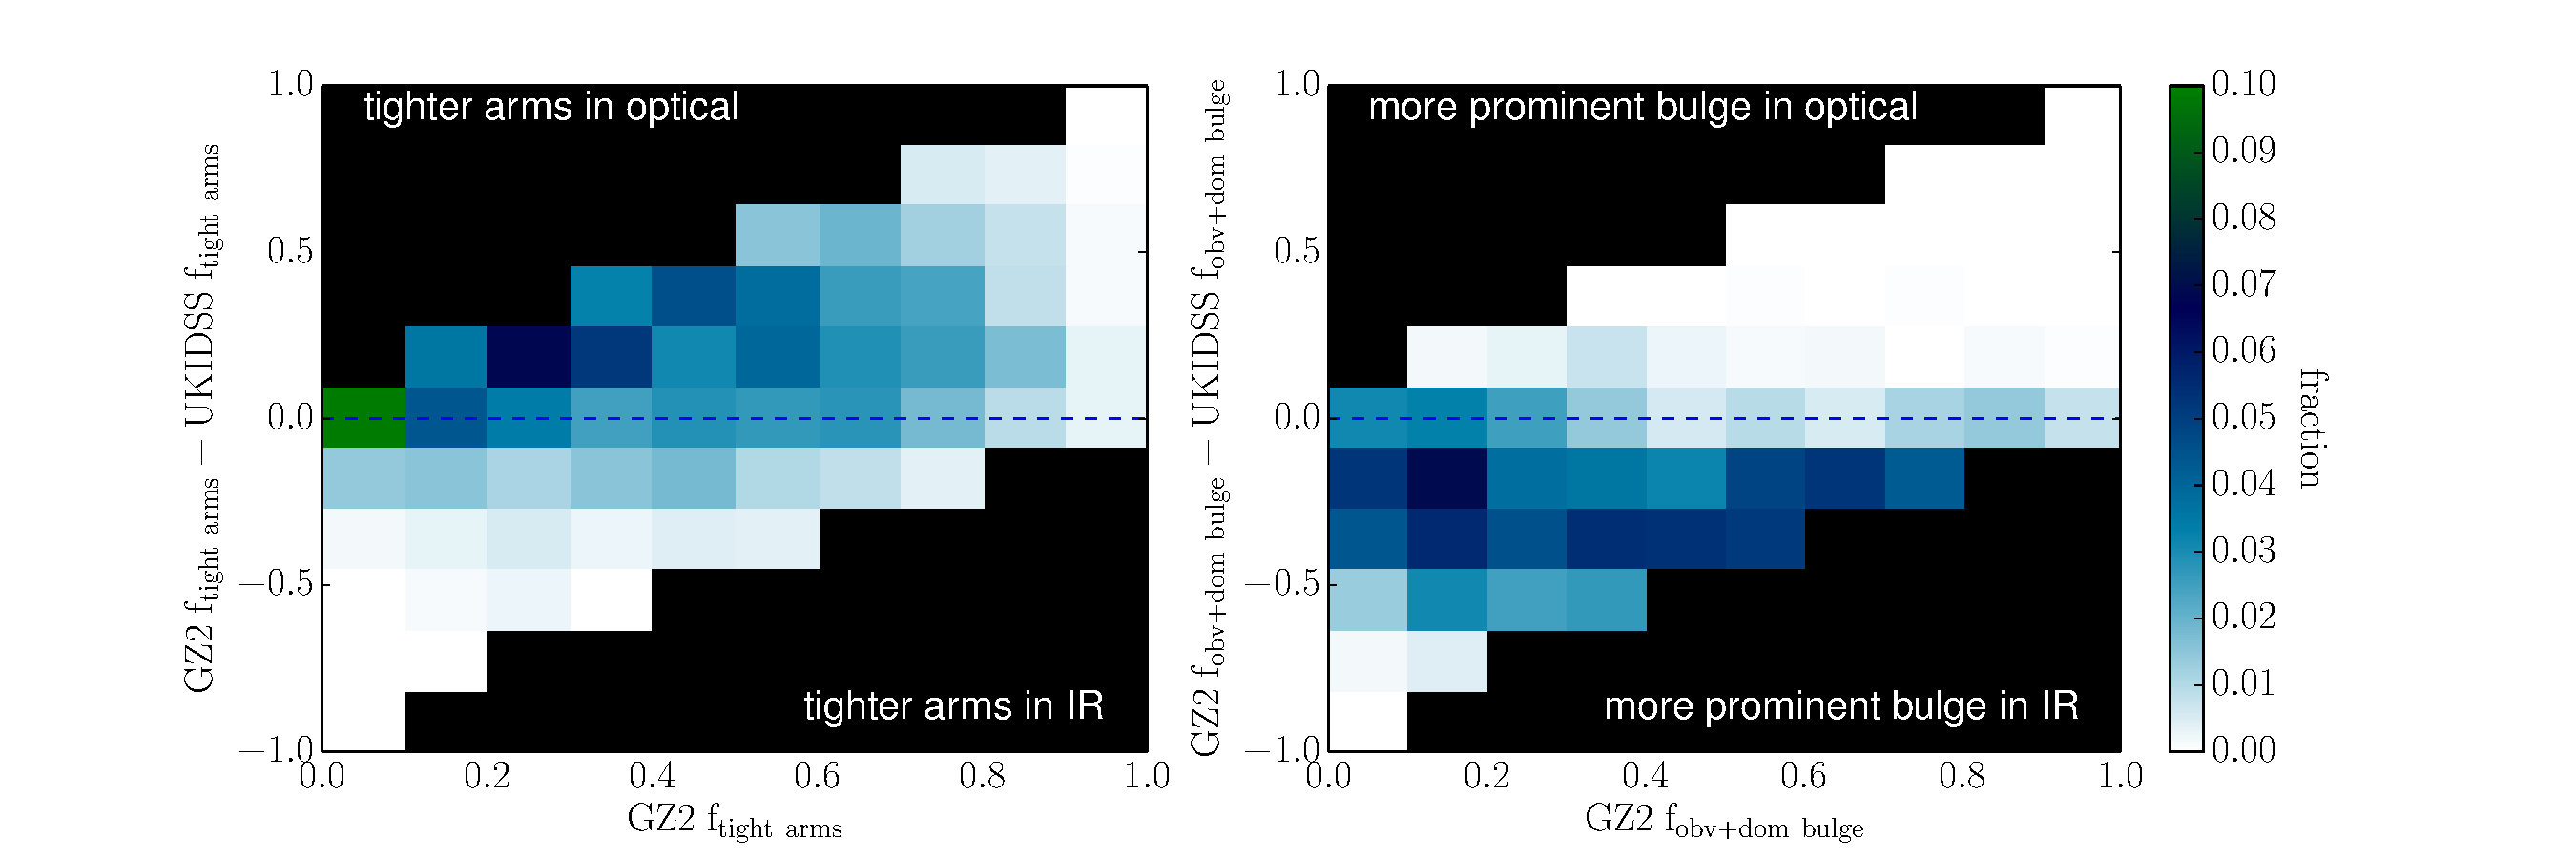
\includegraphics[width=1\textwidth,trim={4cm 0cm 4cm 0cm},clip]{figures/t_type.pdf}
\caption{IR images of galaxies tend to have a looser appearance of arms and more prominent bulges than in optical images. Shown is the difference between optical and IR $\rm f_{tight~arms}$ as a function of optical/GZ2 $\rm f_{tight~arms}$ (\textbf{left}), and difference between optical and IR $\rm f_{obv+dom}$ as a function of optical/GZ2 $\rm f_{obv+dom}$ (\textbf{right}) for 502 galaxies which were classified as spiral in both IR and optical images. The colors represent the fraction of galaxies that populate any given bin, and bins which could not represent a possible difference in vote fraction ($\Delta f > f$ or $\Delta f < f-1$) are colored black. The blue dotted line in both represents a difference in vote fraction of 0, such that galaxies above the line have larger IR vote fractions for the feature represented in each plot, respectively.}
\label{fig:ttype}
\end{figure}

So far the appearance of spiral arms visible in both the optical and infrared have been compared; on average, GZ infrared morphologies are slightly earlier than the optical, a result of a looser appearance of the arms and more prominant bulges. But what of the the optically spiral galaxies whose arms disappear in the IR? Of the 959 optical spirals in the volume and S/N limited sample, 279 (29\%) of these were not classified as spirals in the IR. These types will be hereafter referred to as SONIs (Spiral in Optical but Not Infrared) for convenience. The most common morphological classes of galaxies which do not exhibit spiral arms are ellipticals, S0s, and edge-on disks (which may or may not truly have spiral arms, but cannot be discerned due to orientation angle). This section will explore which of these classes SONIs tend to occupy in the IR. 

Figure~\ref{fig:sankey} shows the different pathways galaxies in the UKIDSS sample follow through the decision tree. The left flow diagram shows the breakdown of morphologies of all galaxies in the volume-limited sample, while the right diagram includes only the SONIs. Galaxies which follow the spiral pathway must first be classfied as featured (T00), then not edge-on (T01). At this point the not edge-on featured galaxies can follow the 'spiral' or 'not spiral' path (T03). Those marked as spirals are classified by how tight the arms appear (T09) and how many arms are present (T10). Last, both the spirals and not-spirals are classified by bulge prominence (T04). As a result of this type of decision tree, there are several pathways galaxies may take to ultimately obtain a ``not spiral'' classification. They may be classified from the beginning as not featured (as ellipticals or star/artifacts), or they may be featured but edge-on, or they may be featured and not edge-on, and still show no spiral arms.

The diagram on the right shows which of these paths SONIs tend to take, resulting in their ultimate classification of ``not spiral'' in the IR. 72\% of SONIs follow the elliptical path; that is, the optically-visible spiral arms must become so faint that all that can be seen is the central bulge, which by eye becomes discernable from a full spheroidal galaxy. 19\% are classified as both featured and not edge-on. One might hypothesize a majority of these exhibit stellar bars, which drives the ``featured'' classifications when there are no spiral arms to do so. However, there is no excess of strong bars detected; only 24\% of the not edge-on featured SONIs are strongly barred, which is actually lower than that of the full sample (33\%). Since the diagram flows are determined by a plurality of votes for each Task, however, the possibility of weak bars of driving the ``featured'' classification is not accounted for here. Therefore most of the galaxies on this path are likely either weakly barred, and/or retain evidence of both an underlying disk and a bulge, with enough contrast to keep them from being classified as purely elliptical. However it is clear that the bulge is very close to dominating the total light distribution in many of these galaxies; for SONIs, 89\% are classified as having an either obvious or dominant bulge, as compared to 82\% showing obvious or dominant bulges in the full sample. 



\begin{figure}
\centering
\includegraphics[width=1\textwidth]{figures/sankey.pdf}
\caption{Flow diagram showing the breakdown of morphologies in the UKIDSS sample. \textbf{Left}: 15,491 galaxies in the volume-limited sample. \textbf{Right}: 2,346 SONIs: galaxies which were classified as spiral in the optical GZ2 classifications but do not follow the spiral path in the UKIDSS classifications.}
\label{fig:sankey}
\end{figure}

\begin{figure}
\centering
\includegraphics[width=\textwidth,trim={5cm 1cm 5cm 1cm},clip]{figures/smooth_sonis.pdf}
\caption{Example images of galaxies which were classified as spiral in optical GZ2 classifications but followed the ``smooth'' path in the UKIDSS classifications.}
\label{fig:smooth}
\end{figure}

\begin{figure}
\centering
\includegraphics[width=\textwidth,trim={5cm 1cm 5cm 1cm},clip]{figures/notedgeon_sonis.pdf}
\caption{Example images of galaxies which were classified as spiral in optical GZ2 classifications but followed the ``featured, not edge-on, no spiral'' path in the UKIDSS classifications.}
\label{fig:notedgeon}
\end{figure}

 
\begin{figure}
\centering
\includegraphics[width=\textwidth,trim={5cm 1cm 5cm 1cm},clip]{figures/edgeon_sonis.pdf}
\caption{Example images of galaxies which were classified as spiral in optical GZ2 classifications but followed the ``featured, edge-on'' path in the UKIDSS classifications.}
\label{fig:edgeon}
\end{figure}

 
\begin{figure}
\centering
\includegraphics[width=\textwidth,trim={5cm 1cm 5cm 1cm},clip]{figures/artifact_sonis.pdf}
\caption{Example images of galaxies which were classified as spiral in optical GZ2 classifications but were classified as star/artifact in the UKIDSS classifications.}
\label{fig:artifact}
\end{figure}


\section{Bar Fraction}
A clean separation of barred and unbarred galaxy populations is required to properly analyze the various effect bars may have on their host galaxies. If a significant portion of bars are better detected in one waveband than another, both classifications should be incorporated to improve the separation of barred and unbarred samples. This section will investigate whether this should be a necessary process for bar population studies by computing the relative numbers of bars detected in optical and infrared imaging. To avoid possible confusion in this portion of the text, two similar quanities are defined explicitely here: the \emph{bar fraction} is defined as the ratio of barred galaxies to total galaxies in a sample, and $\rm f_{bar}$ is the \emph{bar vote fraction}, which is the fraction of users who detected a bar in an image of an \emph{individual galaxy}.

Barred galaxies in the GZ2 and UKIDSS samples are identified using the same prescription described in Chapter~\ref{chap:baragn} \citep{Galloway2015}. Cuts are placed on $f_{\rm features} \ge 0.35$ and $f_{\rm not edge-on} \ge 0.6$ to limit the sample to featured, not edge-on galaxies. An additional cut is placed on the number of people to answer the bar question $N_{\rm bar}\ge 10$ to ensure adequate statistics in calculating the bar vote fraction $f_{\rm bar}$. Of the galaxies meeting these criteria, bars are then defined as present in galaxies with $f_{\rm bar}\ge 0.3$.  

%To measure the fraction of barred galaxies, the sample is first limited to galaxies for which there were at least 10 answers to the question in the decision tree that asks, ``Is there a sign of a bar feature through the center of the galaxy?'' This cut serves two purposes: first, it provides adequate statistics in computing $\rm f_{bar}$ for each galaxy (see Figure stats). Second, for the UKIDSS sample which has at maximum 40 total classifications per galaxy, this places an indirect cut on the preceding vote fractions $\rm f_{features} \ge 0.25$ and $\rm f_{not~edge~on} \ge 0.25$. This intrinsically limits the sample to featured, not edge-on galaxies, which is precisely the sample desired for computing the bar fraction, as bars are nonexistant in elliptical galaxies, or indetectable in highly-inclined edge-on galaxies. For the GZ2 sample, however, a significant portion of the galaxies have between 40-60 total classifications; so, a cut of $\rm N_{bar} \ge 10$ would not guarantee the same minima for the preceding vote fractions. Therefore direct cuts of $\rm f_{features} \ge 0.5$ and $\rm f_{not~edge~on}$ are additionally placed on the GZ2 classifications to ensure the same sample selection for both wavelengths.  


\begin{figure}
\centering
\includegraphics[width=.75\textwidth]{figures/bar_bar_bar.pdf}
\caption{The middle bar displays the 421 galaxies which are classified as barred in both GZ2 and UKIDSS. To the left shows the number of galaxies classified as barred in GZ2 but \emph{not} UKIDSS (blue). From left to right, these are broken down by those who changed classifications because they followed the smooth path, featured, edge-on path, and featured, not edge-on path (but with insufficient votes at the bar question to allow a barred classification), respectively. To the right shows the number of galaxies classified as barred in UKIDSS but \emph{not} GZ2 (red). These are broken down in the same way as described for the GZ2-classified bars. }
\label{fig:barbarbar}
\end{figure}

\begin{figure}
\centering
\includegraphics[width=\textwidth]{figures/sankey_bar.pdf}
\caption{\textbf{Left}: Flow diagram of UKIDSS-barred galaxies through the first three GZ2 tasks. \textbf{Right}: Flow diagram of GZ2-barred galaxies through the first three UKIDSS tasks. Most UKIDSS-barred galaxies are classified as featured, not edge-on galaxies in GZ2. Those which change classifications to unbarred in the optical do so at the bar question; 22\% of these have vote fractions lower than the threshold $f_{bar}\ge0.3$ required for bar classification.  Similar is true for GZ2-barred galaxies, although $\sim30\%$ change classifications to unbarred in the IR because they initially follow the ``smooth'' path or ``featured, edge-on'', without making it to the bar question in the first place. Of those which reach the bar question, 25\% do not achieve significant bar votes ($f_{bar}\ge0.3$) to allow a bar classifiation.  }
\label{fig:sankeybar}
\end{figure}

Figure~\ref{fig:barbarbar} shows the number of barred galaxies in GZ2 and UKIDSS. Of the 1,102 total bars detected, 672 (61\%) were detected in UKIDSS, and 899 (81\%) were detected in GZ2. The optical data recovers a larger portion of the total bars than the IR data, yet still fails to detect 20\% of them. Due to the structure of the Galaxy Zoo decision tree, there are two ways in which a galaxy would fail to achieve a bar classification: first, its bar vote fraction $f_{\rm bar}$ can fail to meet the threshold cut of $f_{\rm bar}\ge0.3$; these galaxies have reached the bar question and thus are seen as face-on disks, but no bar is visible. Second, the bar question may never be asked of the galaxy in the first place if it is classified as ``smooth'' via the first question, or, classified as ``featured'' but also ``edge-on'' in the second. For galaxies which are classified as barred in one waveband but not the other, it may be helpful to discern via which scenerio they are changing classifications. In the first case, the images would look mostly similar in terms of the overall structure, but the bar would too weak, or perhaps even be masked, to meet the $f_{\rm bar}$ threshold required. In the second case, the images must transform significantly to follow entirely different paths through the tree. 

Figure~\ref{fig:sankeybar} shows path followed by the barred galaxies. On the left is the path of the 672 UKIDSS-barred galaxies through the GZ2 classifications, on the right is the path of the 899 GZ2-barred galaxies through the UKIDSS classifications. For the UKIDSS-barred galaxies, the majority (93\%) of them maintain the same featured, not edge-on morphologies in both wavebands, but change classifications once they reach the bar question. For the GZ2-barred galaxies, a larger fraction of them change classifications earlier, with 16\% of them being classified as smooth from the first question. It is also slightly more common for these galaxies to be re-classified as edge-on in the GZ2 track, but the majority (79\%) are consistent in their featured, not edge-on morphologies, and 34\% of these change classifications from GZ2-barred to UKIDSS-unbarred at the bar question. The numeric breakdown of these distributions is visualized in Figure~\ref{fig:barbarbar}, and example images for each category are shown in Figures~\ref{fig:ubarnogbar} and ~\ref{fig:gbarnoubar}.

\begin{figure}
\centering
\includegraphics[width=\textwidth,trim={0cm 1cm 0cm 1cm},clip]{figures/ubar_no_gzbar.pdf}
\caption{Galaxies classified as barred in UKIDSS (top row, IR images) and unbarred GZ2 (bottom row, optical images). The left column is an example of a galaxy which was not classified as barred in GZ2 because it followed the smooth GZ2 path, the middle followed the featured, edge-on path, and the right followed the featured, not edge-on path.}
\label{fig:ubarnogbar}
\end{figure}


\begin{figure}
\centering
\includegraphics[width=\textwidth,trim={0cm 1cm 0cm 1cm},clip]{figures/gbar_no_ubar.pdf}
\caption{Galaxies classified as unbarred in UKIDSS (top row, IR images) and barred GZ2 (bottom row, optical images). The left column is an example of a galaxy which was not classified as barred in UKIDSS because it followed the smooth UKIDSS path, the middle followed the featured, edge-on path, and the right followed the featured, not edge-on path.}
\label{fig:gbarnoubar}
\end{figure}



\begin{figure}
\centering
\includegraphics[width=\textwidth]{figures/ubar_vs_gbar.pdf}
\caption{GZ2 vs UKIDSS bar strengths of 1,107 featured, not edge-on galaxies measured by $f_{\rm bar}$. Galaxies shown must have 10 people answer the bar question, $f_{\rm features}\ge0.35$ and $f_{\rm not~edge-on}\ge0.6$ in both samples. The dotted white lines indicate the threshold value for bar classification $f_{\rm bar}\ge0.3$; the top-right region therefore displays the fraction of galaxies classified as barred in UKIDSS and GZ2, the bottom left are those classified as unbarred in both, the top-left are UKIDSS-barred and GZ2-unbarred, and the bottom-right are GZ2-barred and UKIDSS-unbarred. Most galaxies have consistent classifications (76\% are either barred in both or barred in neither), 11\% are barred in UKIDSS but not GZ2 (top left) and 13\% are barred in GZ2 but not UKIDSS (bottom right). } 
\label{fig:ubarvgbar}
\end{figure}

Most galaxies which change bar classifictions do so \emph{at} the bar question, rather than tending to follow entirely different pathways through the GZ decision tree. Here the change will be analyzed in more detail: Figure~\ref{fig:ubarvgbar} compares $f_{\rm bar}$ measured in UKIDSS and GZ2 for galaxies which were consistently classified as featured and not edge-on in both samples. White dashed lines mark the threshold value for bar identification, $f_{\rm bar}\ge 0.3$. Galaxies to the right of the vertical dashed line were classified as barred in the optical images, and those above the horizontal dashed line were classified as barred in the IR images. Four regions can be defined in this way: The top right region of the plot represents galaxies classified as barred in both wavebands, the bottom right shows those which are unbarred in both, the top left shows those which are barred in the IR but not the optical, and the bottom right shows those which are barred in the optical but not IR.  

The bar vote fraction $f_{\rm bar}$ is well-correlated in both projects. The data follow a mostly 1:1 relationship with an average scatter of $\Delta f_{\rm bar} = +/- 0.1$, resulting in consistent classfications for the majority of galaxies, with 42\% being barred in both and 23\% being unbarred in both. 11\% are barred in UKIDSS but not GZ2 (top left). These tend to not be very strongly barred in UKIDSS, with typical bar vote fractions of 0.3-0.6. Since many of these only barely pass the threshold cut, statistical error is likely a partial driver of the different classifications. 13\% are barred in GZ2 but not UKIDSS; these have a wider spread of bar vote fractions in GZ2, up to $f_{\rm bar,GZ2}\sim0.9$. This change is much more drastic, indicating that the change in classifications in these cases is more driven by a significant differences in the appearance of the images. 

\section{Discussion}

\section{Conclusions}

The main findings of this analysis are as follows:

\begin{itemize}

\item For galaxies whose spiral arms are detected in both optical and IR images, the IR classifications are slightly earlier than the optical, driven mostly by a stronger appearance of the bulge and partly by a looser appearance of spiral arms. 

\item A significant fraction (29\%) of galaxies were classified as having spiral arms in the optical images but not the infrared images. The majority of these (72\%) instead appeared elliptical, 7\% appeared featured but edge-on, and 19\% appeared featured and face-on.

\item For galaxies which can be identified as featured and not edge-on, a majority of 76\% galaxies have consistent barred or unbarred classification in opitcal and infrared classifications. Galaxies which were barred in UKIDSS but not GZ2 tended to be weakly so, such that statistical error is likely the driving factor between the mis-matched classifications. It is more common for bars to be detected in GZ2 but not UKIDSS due to genuine differences in the images, where separation between features were more distinct in the optical and smoothed-over in the IR. 


\end{itemize}


% CHAPTER:  1
% (Note: cannot have a footnote on a word within the \chapter{} construct, it does not work)
\chapter{GZH red disk fraction}
\label{chap:gzh_red_disks}

It is well known that most galaxies tend to exist in one of two populations: blue, late-type disks exhibiting active star formation, and red, early-type ellipticals showing little to no signs of recent star formation \citep{Strateva2001,Baldry2004}. The division between the two color populations is quite distinct when visually represented on a color-magnitude (CMD) or color-color diagram. As shown in the CMD in Figure~\ref{fig:CMD}, galaxies tend to populate in one of two regions: the ``red sequence'' in the upper band, which contains predominently early-type galaxies, and the ``blue cloud'' in the lower, containing mostly late-type spirals. This bimodality in the color-morphology relationship of galaxies has been so widely accepted that color is often used as a proxy for morphological classification in large samples of galaxies (e.g. \citet{Cooray2005,Lee2007,Salimbeni2008,Simon2009}), where expert visual classification is not feasable on such scales (see also: Chapter~\ref{chap:methodology}), while color measurements are more easily available. 

\begin{figure}
\centering
\includegraphics[width=0.75\textwidth]{figures/cmd.png}
\caption{cmd figure}
\label{fig:CMD}
\end{figure}


The relatively tight correlation suggests an evolutionary link between a galaxy's dynamical history (traced by its morphology) and stellar content (traced by its color). In the simplest interpretation, it could be deduced that galaxies tend to begin their lives as young, star-forming disks, until some mechanism (secular or external) causes star-formation to cease while the galaxy simultaneously undergoes a morphological tranformation from disk to spheroidal. 

The advent of larger surveys and more reliable methods for measuring morphology (independently of color) has allowed for more nuanced interpretations of the simple model. For instance, the degree of incompleteness in the color-morphology relationship is now much more realized, with the recent identifcations of significantly large samples of red spirals and blue ellipticals. Using morphological classifications from GZ1, \citet{Masters2010} found 6\% of a sample of $\sim$5000 spirals to be red; similarly, \citet{Schawinski2009} found 6\% of early-type galaxies to be blue. The existence of these objects may represent transition phases in the pathway from the blue cloud to the red sequence, and also give insight into what processes may quench or initiate star-formation without inducing a morphological change, or visa versa.

Another probe for understanding the transition from blue cloud to red sequence is the ``green valley'', the intermediate region between the two. In addition to the ellipticals in the blue cloud and spirals in the red sequence, galaxies of all types residing in the green valley were thought to represent the transition stages of this evolutionary pathway. The intermediate colors in this region indicate a recent quenching of star-formation \citep{Martin2007,Salim2007}, and the dearth of galaxies here (as compared to the high populations in the red sequence and blue cloud) initially suggested that the quenching process initiating transition across the CMD is very rapid.

A closer look at the populations within the green valley show that the processes causing galaxies to evolve from the blue cloud to red sequence may be very different. \citet{Schawinski2009} studied the morphological distribution (measured by the GZ1 project) of $\sim$4000 green-valley galaxies, finding that late-type and early-types likely go through two different evolutionary tracks. For late-types, the quenching process is gradual, and initiated by a cutoff of a gas reservoir. Galaxies quenched recently in this way would populate the green valley at $z=0$, and those which quenched at an earlier time would be currently identified as red passive disks. Whether these red disks continue to evolve into spheroidals via some process after the initial quenching is unclear from a local Universe analysis. For early-types, the quenching is rapid and probably external and violent, thus triggering the morphological change from disk to spheroidal.  

Analysis of the color-morphology relationship in the local Universe has revealed a close but imperfect bimodality as well as proposed mechanisms by which galaxies undergo different quenching processes, driving their evolution along the CMD. Even more may be revealed by studying the different populations as a function of cosmic time, which is becoming more possible with the data from large high-redshift surveys such as COSMOS and deep imaging via HST-ACS. It has been established now, for instance, that the bimodality does exist out to $z\sim1$ \citep{Bell2004,Cirasuolo2007,Mignoli2009} and possibly beyond \citep{Giallongo2005,VanDokkum2006,Franzetti2007,Cassata2008}. What requires further study is how exactly the proportions change at different epochs.

\section{Sample Selection}
\label{sec:reddisksample}
info to include:
cross match with ultravista for rest-frame colors, volume limit, morphological cuts (pfeatures, pclumpy, pedgeon)

\section{Galaxy Classification: Identifying the Passive Population}
\label{sec:colorcolor}
To classify the galaxies as quiescent or star-forming, a method similar to that described by \citet{Ilbert2013} (hereafter I13) was used, which implements a rest-frame NUV-$r^{+}$ versus $r^{+}$-J diagnostic. Here are some reasons these colors are great (NUV-r:) \citep{Arnouts2007a,Salim2005a,Wyder2007},\citep{Martin2007}

The demarcation line to separate the quiescent and active populations at $z=1$ is adopted from I13, which defines the quiescent galaxies as those which satisfy: $M_{NUV}-M_{r^{+}} > 3(M_{r^{+}}-M_{J})+1$ and $M_{NUV}-M_{r^{+}} > 3.1$. I13 applies this criteria to all galaxies in a range of $0.2<z<3$, although it performs best at separating the two populations in the redshift bin $0.7<z<1.2$, where $>98\%$ of galaxies identified as quiescent exhibited star formation rates less than $log(SFR) = -11$ (see Figure 3 of I13). Therefore this work uses the I13 separation criteria at $z=1$, and computes the evolution of the demarcation lines as a function of redshift to $z=0$. 

The evolution of $r-J$ and $NUV-r$ colors was measured using a stellar population synthesis model from \citet{Bruzual2003}. An instantanious-burst model (ssp) was chosen from the Padova1994 track to represent the color evolution of a passively evolving galaxy, with a metallicity $Z=0.008=.4Z_{\sun}$, which is the typical metallicity of passive galaxies with mass $9 < log(M_{*}/M_{\odot}) < 10$ (\citet{Peng2015}, Figure 2a), chosen to correspond to the median mass of the sample ($log(M_{*}/M_{\odot})=9.7)$. Figure~\ref{fig:bcmodel} shows the evolution of the two colors as a function of redshift, where the single starburst at $t=0$ was placed at $z=6$. A linear relationship was fit to the data within the range $0<z<2$, and the slope was used to redefine the demarcation lines in five redshift bins: one with central value $z=0.007$ (used to classify the SDSS ferengi2 sample), and four with central values $z$ = [0.30,0.50,0.70,0.90] with widths $\Delta z=0.2$. The quiescent galaxies are thus defined in these bins as those that satisfy:

\begin{equation}
M_{NUV}-M_{r^{+}} > 3.1 + a_{1}(z)
~\rm and~
M_{NUV}-M_{r^{+}} > 3(M_{r^{+}}-M_{J} + a_{2}(z))+ a_{1}(z) + 1  
\end{equation}

where $a_{1}(z) = [0.54,0.38,0.27,0.16,0.05]$ and $a_{2}(z) = [0.19,0.14,0.10,0.06,0.02]$. 

\begin{figure}
\centering
\includegraphics[width=\textwidth]{figures/hr_m52_evo.pdf} 
\caption{Evolution of colors using stellar population synthesis models. Galaxy was assumed to have formed at $z=6$ for plotting purposes.}
\label{fig:bcmodel}
\end{figure}

\section{Using Ferengi2 to correct for incompleteness in the red disk fraction}

described in previous section that it's difficult or impossible to disentangle whether a small vote fraction of \ffeatures corresponds to galaxies which are intrinsically smooth, or whose features have been washed out at high redshift. So while we can't correct the vote fraction for unique galaxies, we \emph{can} estimate the \emph{number} of disk galaxies we would fail to detect at a given redshift. 

To account for this incompleteness in disk detection, a correction factor $\xi$ is applied. This is defined as the number of disks detected divided by the true number of disks expected to exist in a given redshift interval: $\rm \xi(z)=N_{detected}/N_{true}$. Acknowledging that the completeness in disk detection may depend on galaxy color, the corrected red disk fraction can be calculated as:

\begin{equation}
f=\frac{N_{RD}\times \xi^{-1}_{red}}{N_{RD}\times \xi^{-1}_{red} + N_{BD} \times \xi^{-1}_{blue}}
\label{eqn:reddiskfraction}
\end{equation}

If there is no color bias in disk detection, $\xi_{red}=\xi_{blue}$, and this term cancels out, leaving the fraction unchanged. If there is a bias, however, the $\xi$ terms do not cancel, and the incompleteness in disk detection could have a large effect on the red disk fraction. Therefore a careful measurment of $\xi$ is estimated for both red and blue disk galaxies using the \ferengi2 set of simulated images.

\ferengi2 is the set of images created from 936 nearby ($z<0.01$) galaxies that were artificially redshifted to 8 redshifts between $z=0.3$ and $z=1$, giving a total of 7,488 simulated images (the sample is described in detail in Chapter~\ref{chap:ferengi}). The images were classified in Galaxy Zoo using the same decision tree as used for Galaxy Zoo Hubble. 134 highly inclined disk galaxies were removed from the sample by excluding any with $N_{edgeon}>20$ and $f_{not~edge-on}>=0.6$, using the vote fraction associated with the real galaxy image measured in GZ2. This cut was shown in Chapter~\ref{chap:baragn} to correlate well with inclination angle $cos(a/b)<67^\circ$. This was to exclude those which may be mis-classified due to dust-reddening (see section~\ref{sec:reddisksample}).  Using the NUV-J-R selection method described in section~\ref{sec:colorcolor}, the remaining sample was divided into a set of red sequence galaxies (259 per redshift bin) and blue cloud (543 per each redshift bin), shown in Figure~\ref{fig:ferengi2colorcolor}.
 

\begin{figure}
\centering
\includegraphics[width=.6\textwidth,trim={.5cm 0cm .5cm 0cm},clip]{figures/ferengi2_colorcolor.pdf}
\caption{Separation of the quiescent population (red sequence) and active population (blue cloud) of the \ferengi2 sample.}
\label{fig:ferengi2colorcolor}
\end{figure}


The completness values $\xi_{red}(z),\xi_{blue}(z)$ were then computed in varying bins of redshift for the red sequence and blue cloud galaxies separately. An example calculation of $\xi_{blue}$ in the $z=0.7$ bin is shown in Figure~\ref{fig:inc_subplot}. Each point represents a \ferengi2 galaxy, where the y-axis indicates the value of \ffeatures~measured in the image redshifted to $z=0.7$, and the x-axis indicates the value of \ffeatures~measured in the same galaxy redshifted to $z=0.3$. Disk galaxies are identified as those for which \ffeatures~$\ge0.3$. Since, on average, \ffeatures~decreases for the same galaxy but viewed at higher redshifts, the number of galaxies meeting this threshold is generally fewer at higher redshifts than lower redshifts. This is indicated by the dotted lines: galaxies to the right of the vertical dashed line at $\rm f_{features,z=0.3}=0.3$ are identified as disks at $z=0.3$; their sum is considered the ``true'' number of disks, $\rm N_{true}$. Similarly, the galaxies above the horizontal line at $\rm f_{features,z=0.7}=0.3$ are identified as disks at $z=0.7$; their sum is the ``detected'' number of disks at $z=0.7$, or $\rm N_{detected}$. As obvious in the figure, $\rm N_{detected}$ is in general much lower than $\rm N_{true}$, emphasizing the increasing difficulty in detecting features at higher redshifts. Their ratio is the completeness $\xi$; in this example $\xi_{blue}(z=0.7)=0.61$, meaning only 61\% of disks were detected at this redshift. 

\begin{figure}
\centering
\includegraphics[width=.65\textwidth]{figures/incompleteness_z7.pdf}
\caption{Example calculation of completeness $\xi$ at redshift $z=0.7$. Points represent \ferengi2 images classified in Galaxy Zoo. The y-axis corresponds to the value of \ffeatures~measured at the galaxy redshifted to $z=0.7$, and the x-axis corresponds to the value of \ffeatures~measured at the galaxy redshifted to $z=0.3$. On average, the \ffeatures~is lower at the higher redshift, indicating users on average have more difficulty identifying features in images at higher redshifts. The dotted lines correspond to \ffeatures=0.3, the threshold above which a galaxy is considered to have a disk. Galaxies to the right of the vertical dashed line were identified as disks at the lowest redshift $z=0.3$, the total number defined as $\rm N_{true}$, the true number of disks. Galaxies above the horizontal dash line were identified as disks at the higher redshift $z=0.7$, the total number defined as $\rm N_{detected}$. The ratio $\rm \xi=N_{detected}/N_{true}$ is the completeness value; in this example, only 61\% of disks were detected at $z=0.7$.}
\label{fig:inc_subplot}
\end{figure}

It was hypothesized that the completeness in disk detection may be a function of other parameters in addition to redshift. At fixed redshift, for example, it is reasonable to guess that features could be easier to detect galaxies that have higher mass, radius, or surface brightness. To test whether these parameters also impact the number of disks detected, the completeness was measured in fixed redshift bins as a function of surface brightness, effective radius, and mass. Surface brightness was measured using \sextractor{} calculations of {\tt MAG\_AUTO}, $b/a$ and $R_{e}$ measured in the \Iband{} band images, in the same way as described in Chapter~\ref{chap:ferengi}. The effective radius used was the 50\% {\tt FLUX\_RADIUS} converted in to kpc, and the masses used were the {\tt MEDIAN} values calculated in the MPA-JHU catalog.

Figure~\ref{fig:xi_v_sb} shows completeness as a function of redshift and surface brightness, for the red sequence and blue cloud galaxies. 8 redshift bins were further divided into bins of surface brightness with varying widths, where the sizes were chosen to satisfy that $N_detected + N_true \ge 10$ in each bin. This was chosen as a comprimise between having a sufficient number of galaxies in each bin to compute the completness fraction $\xi = N_{detected}/N_{true}$, and to have enough bins of surface brightness to measure a trend with confidence of completeness as a function of $\mu$. Visual inspection of the data did not suggest any relationship between the two. To be sure, the data were fit to a linear function in each redshift bin (Figure~\ref{fig:notlinear}). For each fit, a p-value representing a hypothesis test whose null hypothesis is that the slope is zero was computed. Only one reached the criteria $p<0.05$, but with a low $R^{2}$ value of 0.28 which is not considered large enough to represent a good fit. This process was repeated using effective radius and mass as parameters, with the same results. Therefore only redshift was used as a parameter which impacted completeness value with confidence.  


\begin{figure}
\centering
\includegraphics[width=\textwidth,trim={3cm 0cm 3cm 0cm},clip]{figures/xi_v_sb.pdf}
\caption{Completeness $\xi$ as a function of redshift and surface brightness for red sequence (left) and blue cloud galaxies (right).}
\label{fig:xi_v_sb}
\end{figure}

\begin{figure}
\centering
\includegraphics[width=\textwidth,trim={2cm 1cm 2cm 1cm},clip]{figures/notlinear.pdf}
\caption{Completeness $\xi$ as a function of redshift and surface brightness for red sequence (left) and blue cloud galaxies (right).}
\label{fig:notlinear}
\end{figure}


\begin{figure}
\centering
\includegraphics[width=\textwidth,trim={2cm 1cm 2cm 1cm},clip]{figures/completenessmoneyplot.pdf}
\caption{Completeness $\xi$ as a function of redshift moneyplot}
\label{fig:notlinear}
\end{figure}


 

%Conclusion Chapter
%%%%%%%%%%%%%%%%%%%%%%%%%%%%%%%%%%%%%%%%%%%%%%%%%%%%%%%%%%%%%%%%%%%%
% conclusion.tex:
%%%%%%%%%%%%%%%%%%%%%%%%%%%%%%%%%%%%%%%%%%%%%%%%%%%%%%%%%%%%%%%%%%%%
\chapter{Looking Forward}
\label{summary_chapter}

Morphology has been, and continues to be, one of the strongest tools available for unravelling the fundamental aspects of the evolution of galaxies. Understanding the myriad secular and environmental processes which give rise to the multitude of morphological types observed contributes to our growing knowledge of the past, present, and future of our Universe.

Using morphology as such a tool, however, is not without its own challenges. Most of these stem from the difficulty in obtaining accurate morphological classifications on a sufficiently large scale. For example, while the SDSS has imaged the largest number of galaxies in a single survey to date ($N \sim 900,000$), only a small fraction of these are nearby enough, large enough, and bright enough to accurately classify their morphologies. Figure~\ref{fig:simmonsgal} shows side-by-side images of a galaxy at $z=0.1$ imaged by SDSS (left) and HST (right). The ground-based image at 0.4''/pixel is not resolved enough to even make out the strong bar or spiral arms, which are very easy to identify in the HST image at 0.04''/pixel.  
 
\begin{figure}
\centering
\includegraphics[width=.75\textwidth]{figures/simmons_galaxy.jpg}
\caption{Resolution of the instrument has a strong impact on the physical appearance of a galaxy, and large differences could change a morphological classification drastically, even for nearby galaxies. Shown is a spiral galaxy at $z=0.1$, imaged by SDSS at $\sim$.4''/pixel (left), and HST at $\sim$.04''/pixel (right) (HST Program ID 14606, PI: Simmons). The strong bar and distinct spiral arms in the HST imaging are mostly lost in the low-resolution ground-based image. }
\label{fig:simmonsgal}
\end{figure}

The solution to this problem has typically been to limit one's sample to only include the most bright galaxies, via a magnitude or volume-limit, to ensure all morphologies in the study are accurate. However a statistical price is paid, particularly in population studies which seek to identify dominant trends in large samples of galaxies. Such studies tend to require extensive binning of the parent sample to remove inter-dependencies in the variables, which as a consequence increases the statistical error in the results as the number of subjects per bin decreases. This type of limitation amplifies as one extends to higher redshift; even the high-resolution capability of HST is insufficient in capturing consistent detailed morphological substructures for galaxies beyond $z\sim0.5$, except for the very largest and brightest objects.

The future of the field is incredibly promising, as technological advances in instrumentation continue to improve on these limitations. Noteworthy examples include the \href{http://www.gmto.org/}{Giant Magellan Telescope (GMT)}, \href{http://www.eso.org/public/teles-instr/elt/}{Extremely Large Telescope (ELT)}, and the \href{http://www.tmt.org/}{Thirty Meter Telescope (TMT)} which will provide images 10-16 times sharper than HST, due to their improved light-collecting areas via large mirrors and implementation of sophisticated adaptive optics technology. 

Perhaps the most notable upcoming advances in this field involve the \href{https://www.lsst.org/}{Large Synoptic Space Telescope (LSST)} and the \href{http://sci.esa.int/euclid/}{Euclid} mission, which will be imaging galaxies on scales previously unattainable. Producing data on the order of terabytes per night, the surveys are ultimately expected to produce detailed images of more than a billion galaxies. While samples on this scale may certainly solve the afforementioned statistical challenges of morphological population studies, this inflow of data presents an entirely new challenge: how can we possibly obtain accurate morphologies on such a large scale in a reasonable timeframe? On these scales, even crowdsourced visual inspection via Galaxy Zoo is nowhere near fast enough. 

The next stage of Galaxy Zoo is tackling this issue by combining human and machine effort, beginning with an innovative system dubbed Galaxy Zoo Express (GZX) (Beck et al. 2017, submitted). GZX improves on the speed and accuracy of human classifications in two ways. First, it maximizes the information that can be obtained from human effort via the algorithm SWAP (Space Warps Analysis Pipeline) \citep{Marshall2016}. SWAP continuously tracks and updates the probability that a galaxy has a given feature, given the history of the volunteers' classifications and their performance classifying known galaxies as part of a training set. Using this technique, human effort is greatly reduced as most galaxies would not require 40 volunteers all classifying each galaxy, which was the retirement threshold in all previous GZ projects. Second, GZX incorporates a machine-learning algorithm which works together with the human classifications to increase the classification time even further. With all of these improvements combined, Beck et al. 2017 showed that GZX could classify 70\% of the GZ2 catalog in \emph{32 days}, a feat that took a full year using the current approach. 

This thesis began with the observation that all data available for studying the evolution of the Universe is contained in a single snapshot of the present cosmos. Methods of imaging galaxies in this snapshot are continuously advancing, as are methods for fast and efficient morphological classification. These advancements undoubtedly point to a promising new era of discovery, which should unveil a whole new wealth of information to further our understanding of the life and fate of galaxies in the Universe.

So long and thanks for all the fish! 

 



% Bibliography
\bibliography{/home/mel/Documents/Papers/library}  

% Appendices
\appendix

\end{document}
